We work in the smooth category.  All maps and manifolds are $C^\infty$. All surfaces are oriented unless explicitly stated otherwise.

\section{Introduction}

  The first goal of this paper is to introduce a theory of virtual Legendrian knots.  The second goal is to study the group of Vassiliev invariants of virtual Legendrian knots.  We show that this group is naturally isomorphic to the group of Vassiliev invariants of framed virtual knots with fixed Maslov number in the spherical cotangent bundle of a surface.  As a result, Vassiliev invariants do not distinguish virtual Legendrian knots which are isotopic as framed virtual knots and have the same virtual Maslov number.  Similar theorems were proved by Goryunov \cite{Goryunov}, Hill \cite{Hill}, Fuchs-Tabachnikov \cite{f&t}, and Chernov \cite{Chernov} for Legendrian knots in various contact structures. 

% We introduce a theory of virtual Legendrian knots.  By using virtual versions of the Maslov and Bennequin numbers, it is easy to find examples of virtual Legendrian knots that are isotopic as virtual knots but not isotopic as virtual Legendrian knots.  However we do not know whether there are virtual Legendrian knots with the same Maslov and Bennequin numbers, that are isotopic as virtual knots but not as virtual Legendrian knots.   In order to answer this question, one might try to find invariants that can distinguish such knots.  In our theory, every virtual Legendrian knot has a natural framing, and any two virtually Legendrian isotopic Legendrian knots must be isotopic as virtual framed knots.  In this paper, we show that Vassiliev invariants cannot distinguish virtual Legendrian knots that are isotopic as virtual framed knots and have the same virtual Maslov number.  

% Topo isotopic plus same Maslov implies same connected component? Topo isotopic plus same Bennequin implies framed homo?

We give three equivalent formulations of virtual Legendrian knot theory.  The first, which we introduce below, was motivated by the formulation of virtual knot theory given by Carter, Kamada and Saito \cite{CKS}, and was suggested to us by Chernov \cite{ChernovDefn}. Briefly, virtual Legendrian knots are wavefronts on surfaces up to stabilization and destabilization of the surface.

% Namely, Carter, Kamada and Saito showed that the virtual knot theory introduced by Kauffman CITE is equivalent to the following formulation: A virtual knot is a knot diagram on an oriented surface $F$, or equivalently, a knot in a thickened surface $F\times [0,1]$.  Two virtual knots are equivalent if they are related by a sequence of Reidemeister moves on the surface, and stabilizations and destabilizations of the surface.  Destabilizations and stabilizations will be reviewed in the next section.

Suppose that the surface $F$ is made of an isotropic, homogeneous medium, and that light rays are emitted from a point or curve $\omega$ on $F$.  The set of points that these light rays can reach in at most a fixed time $t$ has a boundary.  This boundary is called the {\it wavefront} of $\omega$ after time $t$.  As $t$ increases, the wavefront may no longer be immersed, because semi-cubical cusps may appear.  We say a (cooriented) {\it wavefront} on an oriented surface $F$ is a cooriented curve on $F$ which is immersed except at a finite number of semi-cubical cusps.  The coorientation represents the direction of propagation of the wavefront.  A wavefront is {\it generic} if it has a finite number of self-intersection points, all of which are transverse double points.  


\begin{figure}[htbp]\label{dangerous.fig}
	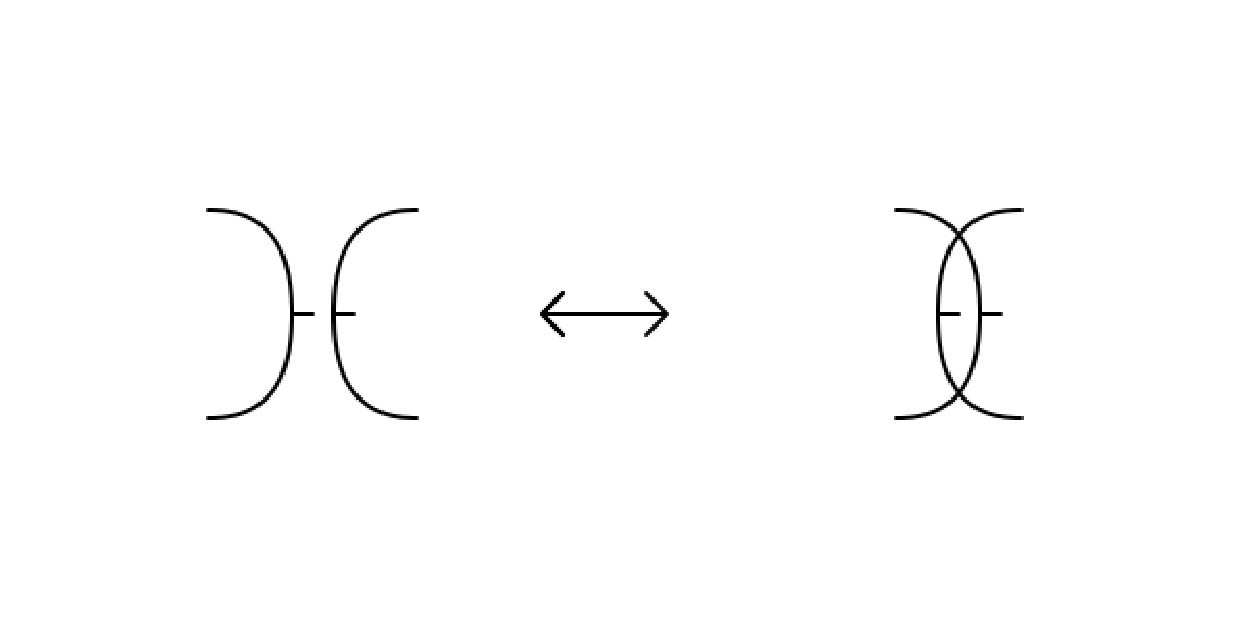
\includegraphics[width=5cm]{dangerousTangencyMove}
	\caption{The dangerous tangency move.}
\end{figure}

The spherical cotangent bundle $ST^*F$ of the surface $F$ is equipped with a natural contact structure.  Arnold observed that, due to the Huygens principle, the propagation of a wavefront on $F$ lifts to a Legendrian isotopy in $ST^*F$ \cite{ArnoldMechanics, ArnoldPDE}.  That is, lifting the wavefront to $ST^*F$ according to the direction of its coorienting vector produces a curve in $ST^*F$ which is everywhere tangent to the distribution of contact planes, and during the propagation of the wavefront, the lift of this curve undergoes an isotopy while remaining tangent to the contact planes.  

In particular the Huygens principle implies that the {\it dangerous tangency move} in Figure \ref{dangerous.fig} cannot appear during the propagation of a single front $\omega$, because if two branches of $\omega$ become tangent during the propagation in such a way that their coorientations match, they must be tangent for all $t$.


Hence the Legendrian liftings of two generic wavefronts are Legendrian isotopic if and only if the wavefronts are related by a sequence of the moves in Figure \ref{wavefrontmoves.fig} up to certain choices of coorientation, in addition to ambient isotopy.  To obtain all the valid choices of coorientation, one should consider the moves in Figure \ref{wavefrontmoves.fig} with all possible choices of coorientations on the branches, {\it except} in the case of the second move, because dangerous tangencies are prohibited \cite{ArnoldInvariants}.

% Arnold observed that wavefronts obey these moves.  He showed that, due to the Huygens principle, the propagation of a wavefront on a surface $F$ lifts to a Legendrian isotopy in the spherical cotangent bundle $ST^*F$. Hence two wavefronts which are not isotopic as Legendrian knots cannot both be obtained by propagation of a single wavefront.  He also noticed that wavefronts cannot pass through a dangerous tangency in general without changing their Legendrian isotopy class, which is why this move is prohibited.

\begin{figure}[htbp]
	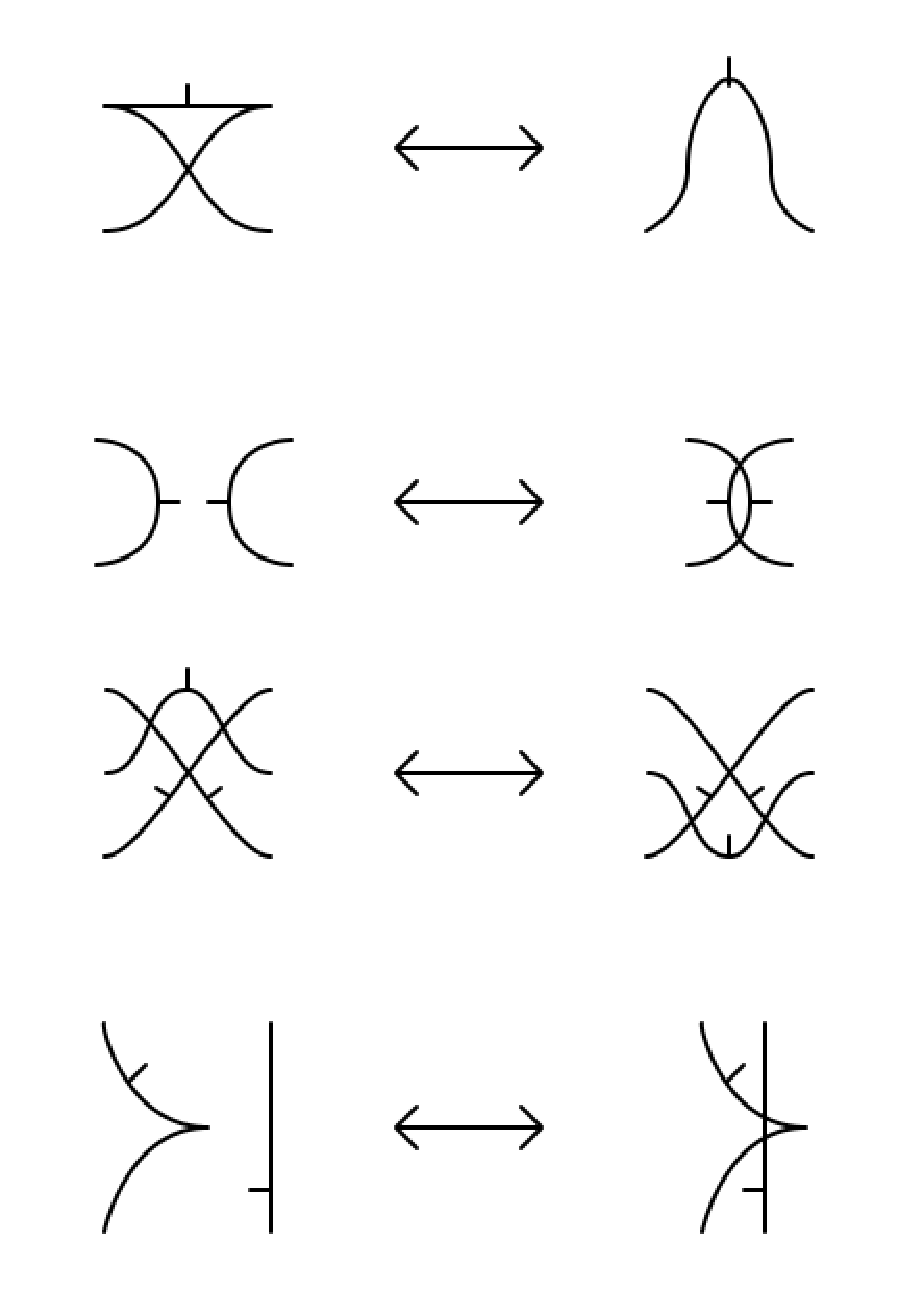
\includegraphics[width=6cm]{wavefrontmoves}
	\caption{Moves for wavefronts on an oriented surface, with one possible choice of coorientation on each branch.}
	\label{wavefrontmoves.fig}
\end{figure}

A virtual Legendrian knot is a wavefront on an oriented surface.  The definition of virtual Legendrian knot theory suggested by Chernov is as follows: two virtual Legendrian knots are equivalent if they are related by wavefront moves and stabilization (addition of handles) and destablization (removal of handles) of the surface. Physically, this corresponds to the notion that the medium through which the wavefront propagates can change its topology outside a neighborhood of the wavefront.


We also give a purely diagrammatic description of virtual Legendrian knot theory.  Namely, one can view a virtual Legendrian knot as a wavefront in the plane with virtual crossings up to certain moves, in the spirit of Kauffman's orginal theory of virtual knots \cite{Kauffman}.  


% If the contact structure $C$ is parallelizable, then one can define the {\it Maslov number} of a Legendrian curve $L$ to be the number of rotations of the velocity vector of $L$ with respect to the chosen frames in $C$.  In $\mathbb{R}^3$ with the standard contact structure, the components of the space of Legendrian curves are enumerated by the Maslov number of the curve, so this condition holds in $\mathbb{R}^3$ with the standard contact structure.  In the solid torus $ST^*\mathbb{R}^2$ the components of the space of Legendrian curves are enumerated by the Maslov number of the curve in combination with the rotation number of its corresponding wavefront in the plane.  




Questions similar to ours have been studied by many people over the last 20 years.  In the rest of this section let $\mathcal{K}\in\{\mathbb{R}, \mathbb{C}\}$ and $\mathcal{A}$ be any abelian group.  In 1997 Fuchs and Tabachnikov \cite{f&t} showed that the vector spaces of $\mathcal{K}$-valued, order $\leq n$ Vassiliev invariants of Legendrian knots with fixed Maslov number in $\mathbb{R}^3$ endowed with the standard contact structure and of framed knots in $\mathbb{R}^3$ are isomorphic.  Around the same time, Goryunov showed that the vector spaces of $\mathcal{K}$-valued, order $\leq n$ Vassiliev invariants of oriented framed knots in the solid torus $ST^*\mathbb{R}^2$ and of oriented plane curves without direct self-tangencies (i.e., wavefronts without cusps) are isomorphic \cite{Goryunov}.


Generalizing the work of Goryunov, Hill \cite{Hill} proved the same result for all planar fronts.  Finally, Chernov \cite{Chernov} was able to show that the groups of $\mathcal{A}$-valued, order $\leq n$ Vassiliev invariants of framed knots in $ST^*F$ where $F$ is any surface, and of Legendrian knots in $ST^*F$ are isomorphic.  


More precisely, suppose $\mathcal{L}$ is a connected component of the space of Legendrian curves in a contact manifold $(M,C)$ and let $\mathcal{F}$ be the connected component of the space of framed curves in $(M,C)$ that contains $\mathcal{L}$.  Chernov proved that the groups of $\mathcal{A}$-valued, order $\leq n$ Vassiliev invariants of framed knots in $\mathcal{F}$ and Legendrian knots in $\mathcal{L}$ are isomorphic for a large class of contact manifolds $(M,C)$.  In particular, the theorem holds for $M=ST^*F$ with its natural contact structure. We develop techniques to show that a similar result holds in the virtual category.
\begin{thm} \label{mainthm}
Let $\mathcal{F}$ be a connected component of the space of virtual framed curves and $\mathcal{L}\subset\mathcal{F}$ be a connected component of the space of virtual Legendrian curves contained in $\mathcal{F}$.  Let $\mathcal{A}$ be an abelian group and $\mathcal{V}_n^\mathcal{F}$ be the group of $\mathcal{A}$ valued Vassiliev invariants on $\mathcal{F}$ of order $\leq n$.  Define $\mathcal{V}_n^\mathcal{L}$ likewise.  Then the restriction map $\phi:\mathcal{V}_n^{F}\rightarrow\mathcal{V}_n^\mathcal{L}$ is an isomorphism.
\end{thm}
It follows that Vassiliev invariants cannot distinguish two virtual Legendrian knots that are homotopic as Legendrian curves and isotopic as framed virtual knots.

\begin{thm}\label{maincor}
Let $x\in \mathcal{V}_n^\mathcal{L}$, $(F_1, K_1), (F_2, K_2) \in \mathcal{L}$ and let $(F_1, K_1)$ be virtually framed isotopic to $(F_2, K_2)$.  Then $x(F_1, K_1) = x(F_2, K_2)$.
\end{thm}

In Section \ref{classical.sec} we discuss virtual version of the Maslov number.  We prove that, as in the classical case, the Maslov number can be used to distinguish virtual homotopic curves that are not virtual Legendrian homotopic.

\begin{thm} Two virtual Legendrian knots are virtual Legendrian homotopic if and only if they have the same virtual Maslov number and are homotopic as virtual knots.
\end{thm}

%TODO: Is this still necessary? --> Polyak \cite{Polyak} 

\section{Flat Virtual Knots}
Virtual knot theory was introduced by Kauffman \cite{Kauffman}.  We will briefly review the definition of a related object, called a {\it flat virtual knot}, or {\it virtual string}, in order to motivate the definition of a virtual Legendrian knot.  Virtual strings were introduced by Turaev \cite{Turaev}.


A virtual string is a counter-clockwise oriented copy of $S^1$, called a {\it core circle}, with arrows whose endpoints are glued to the core circle.  The endpoints of the arrows are required to be distinct.  We identify two virtual strings if there is a homeomorphism from one to the other preserving the directions of the arrows.

Every generic oriented curve on a surface gives rise to a virtual string, called its {\it underlying virtual string}.  To construct the underlying virtual string of a curve, label the double points of the curve $a_1, \dots, a_n$.  Traverse the curve in the direction of its orientation and record the cyclic order in which the labels $a_i$ appear.  Each label appears twice in the cyclic order.  Then mark $2n$ evenly spaced points on a counterclockwise oriented copy of $S^1$, and label these points $a_1, \dots, a_n$ in the same cyclic order in which the labels appear on the double points during the traversal of the curve.  For each $1\leq i \leq n$, connect the two points labelled $a_i$ by an arrow.  The direction of the arrow is determined by the following rule: 

%TODO: I don't understand this rule...

\begin{figure}[ht]
\centering
\subfigure{
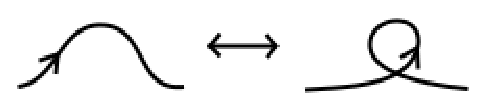
\includegraphics[width=3cm]{R1.eps}
\label{fig:subfig1}
}
\subfigure{
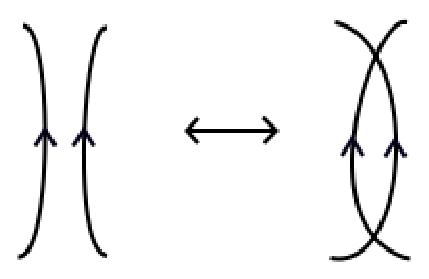
\includegraphics[width=3cm]{R2.eps}
\label{fig:subfig2}
}
\subfigure{
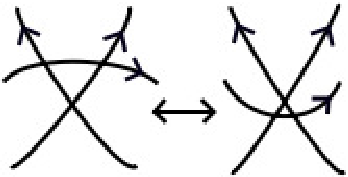
\includegraphics[width=3cm]{R3.eps}
\label{fig:subfig3}
}
\label{fig:subfigureExample}
%\caption[Optional caption for list of figures]{Caption of subfigures \subref{fig:subfig1}, \subref{fig:subfig2} and \subref{fig:subfig3}}
\end{figure}
\begin{figure}[ht]
\centering
\subfigure{
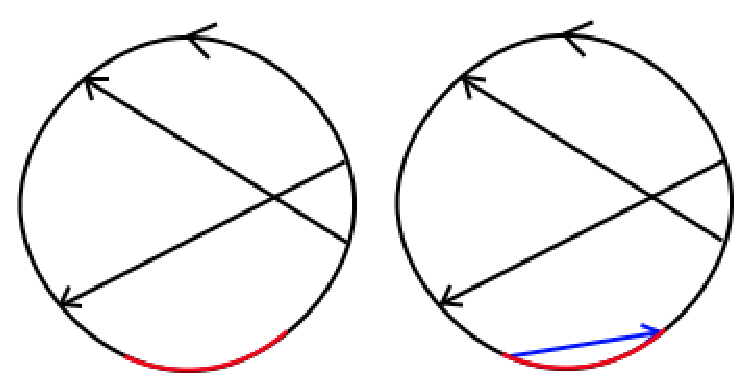
\includegraphics[width=3cm]{R1virtual.eps}
\label{fig:subfig1}
}
\subfigure{
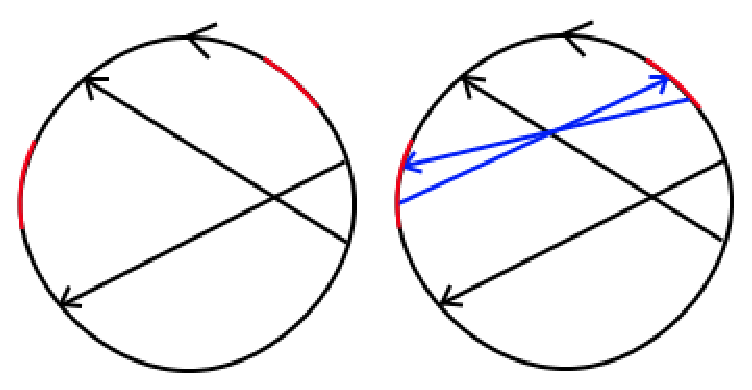
\includegraphics[width=3cm]{R2virtual.eps}
\label{fig:subfig2}
}
\subfigure{
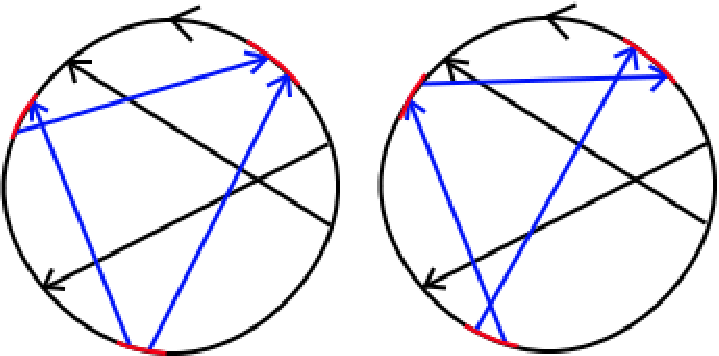
\includegraphics[width=3cm]{R3virtual.eps}
\label{fig:subfig3}
}
\label{fig:subfigureExample}
%\caption[Optional caption for list of figures]{Caption of subfigures \subref{fig:subfig1}, \subref{fig:subfig2} and \subref{fig:subfig3}}
\end{figure}
\section{Virtual Legendrian Knot Diagrams}
A {\it virtual Legendrian knot diagram} is a generic wavefront in $\mathbb{R}^2$ with two types of crossings.  In addition to ordinary wavefront crossings, there are virtual crossings, which are marked with a small circle and obey slightly different Reidemeister moves.  The moves for ordinary wavefront crossings are shown in Figure \ref{wavefrontmoves.fig}.  Again, we can obtain other wavefront moves from these moves by independently reversing the choice of coorientation on any branch, except in the case of the second Reidemeister move, where the dangerous tangency move is forbidden.

The moves involving virtual crossings are pictured in Figure \ref{virtualwavefrontmoves.fig}.  Other moves can be obtained from these moves by independently reversing the coorientation on any branch.  Note that we allow virtual dangerous tangencies.  It is straightforward to check that this definition is equivalent to Chernov's using diagrams similar to Polyak's Gauss diagrams \cite{Polyak} for planar wavefronts.  


%DONE: THERE IS A MISSING MOVE IN FIGURE \ref{virtualwavefrontmoves.fig}, and FIX COORIENTATION ON THE LAST MOVE!!!!!!!!!!
	\begin{figure}[htbp]
		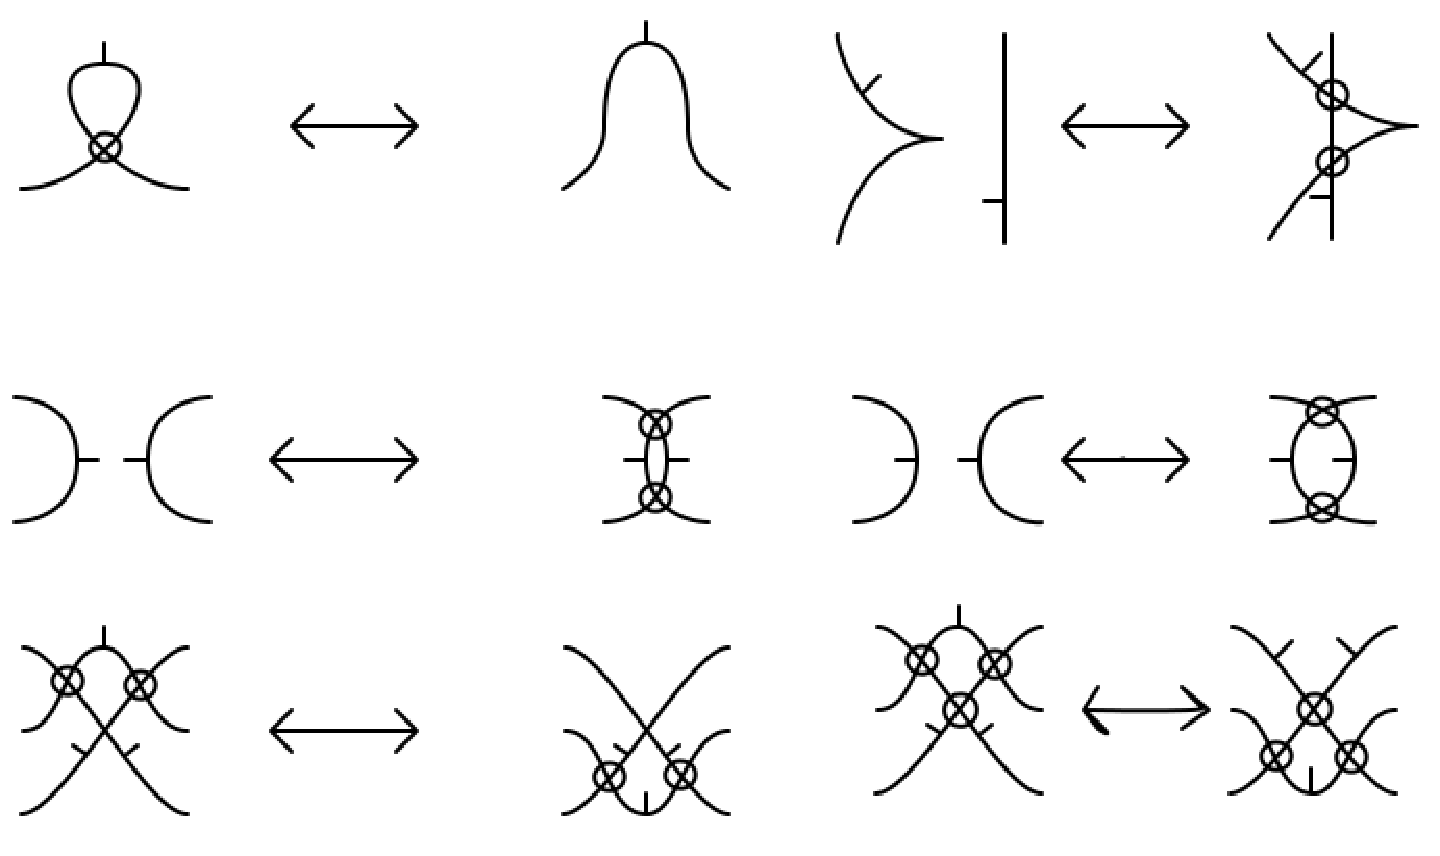
\includegraphics[width=8cm]{virtualwavefrontmoves}
		\caption{Moves for virtual wavefront diagrams in the plane, with one possible choice of coorientation on each branch.}
		\label{virtualwavefrontmoves.fig}
\end{figure}

If we allow the dangerous self-tangency move, the equivalence relation generated is that of {\it virtual Legendrian homotopy}, rather than isotopy.  We sometimes refer to a virtual Legendrian homotopy class as a connected component of the space of virtual Legendrian curves.

\section{Gauss Diagrams for Virtual Legendrian Knots}
We explain how to associate a Gauss diagram to an oriented virtual Legendrian knot.  For planar fronts, our diagrams are similar to the diagrams described by Polyak \cite{Polyak}.  However, unlike Polyak's diagrams, our diagrams are not marked with a basepoint and the signs on our cusps are different from Polyak's.  




The Gauss diagram of an oriented and cooriented virtual Legendrian knot diagram $K$ with $c$ cusps and $n$ crossings (which we assume are transverse double points) is a counter-clockwise oriented copy of $S^1$, with $n$ arrows glued to $S^1$ at their endpoints, and $c$ marked points on $S^1$.  Let $C$ be the set of all marked points.  Each connected component of $S^1\setminus C$ is labeled with a coorientation.  Furthermore we require that the coorientations on adjacent components of $S^1\setminus C$ are different, and as a result $|C|$ is even.  The endpoints of the arrows are distinct, as are the marked points, and no marked point falls on the endpoint of an arrow.  The Gauss diagram of a given front is determined as follows.  We view $S^1$ as the circle parameterizing the curve $K$, and each pair of preimages of a double point of $K$ is connected by an arrow.  At each crossing, we label the outgoing branches of $K$ with a `1' and a `2' so that the ordered pair of their velocity vectors forms a positively oriented frame.  The head of the arrow is placed at the preimage corresponding to the branch labeled `1.'  The marked points of $C$ are the preimages of the cusps of $K$, and each marked point is equipped with a sign as follows.  A cusp of a wavefront is called positive (respectively, negative) if the outgoing branch of the cusp is (respectively, is not) in the coorienting half-plane of the cusp (see Figure \ref{cusps.fig}).  A virtual Legendrian knot diagram and its Gauss diagram are pictured in Figure \ref{Gaussdiagram.fig}.'

\begin{figure}[htbp]
	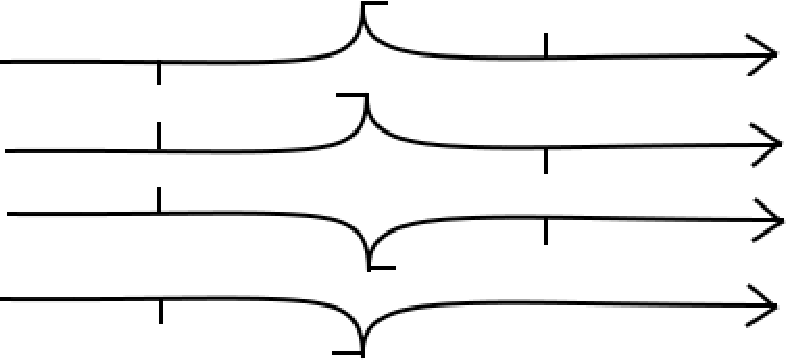
\includegraphics[width=8cm]{goodcusps}
	%TODO: ADD IN MISSING COORIENTATION ON BOTTOM DIAGRAM
	\caption{From top to bottom, a positive left cusp, negative left cusp, positive right cusp, and negative right cusp.}
	\label{cusps.fig}
\end{figure}

\begin{figure}[htbp]
	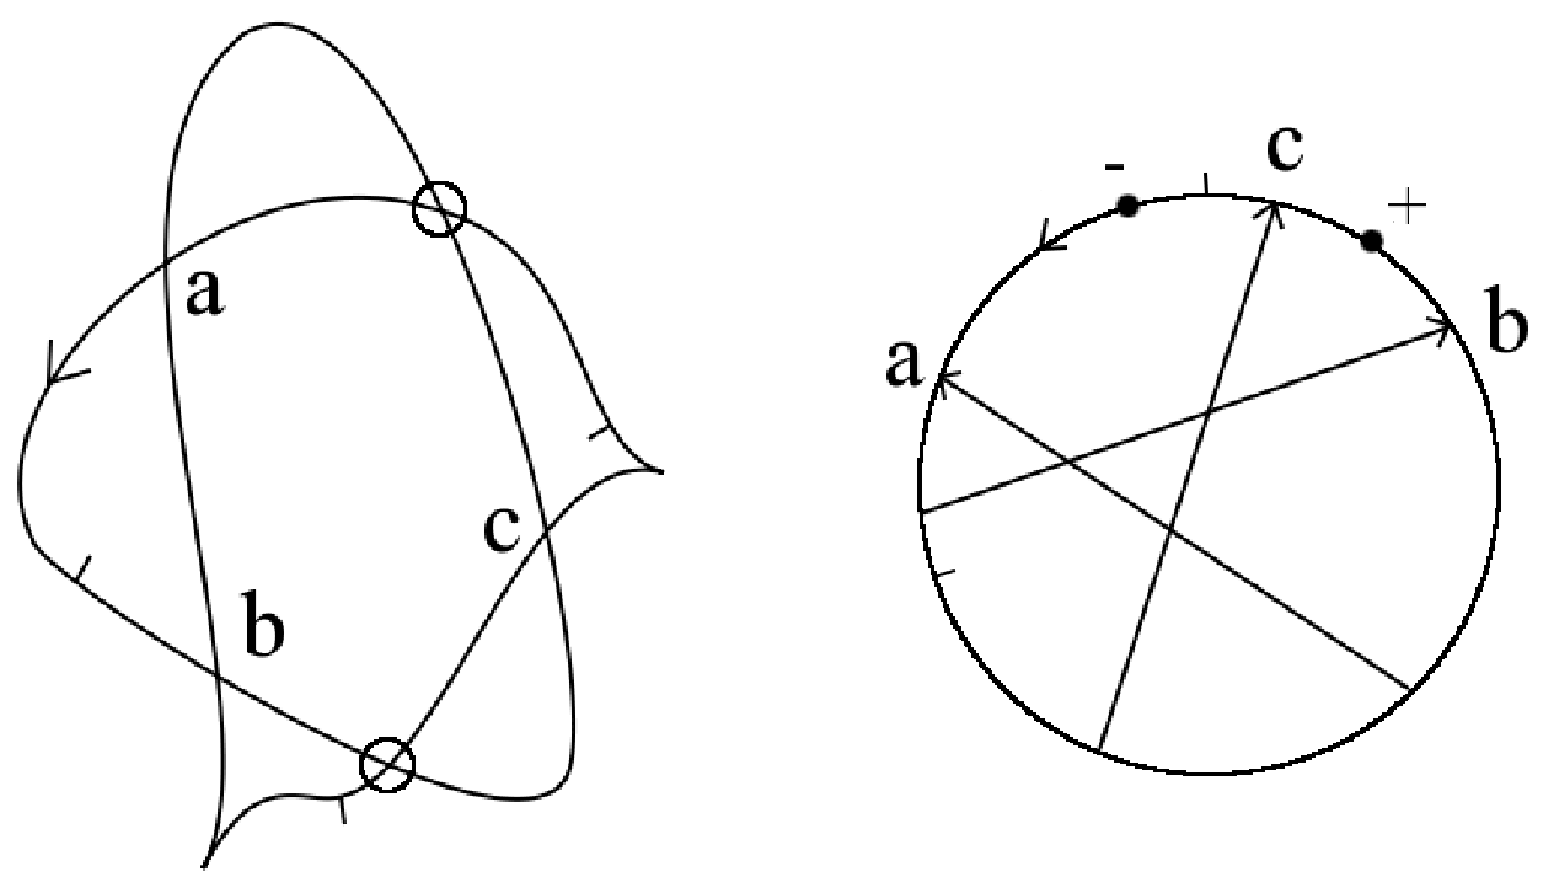
\includegraphics[width=8cm]{Gaussdiagram}
	\caption{A virtual Legendrian knot diagram and its corresponding Legendrian Gauss diagram.}
	\label{Gaussdiagram.fig}
\end{figure}

We can define analogues of front moves on Gauss diagrams. 


\section{Virtual Framed and Legendrian Isotopy in the Spherical Cotangent Bundle}
The goal of this section is to define the notions of virtual framed and virtual Legendrian isotopy.  The definitions in this section are motivated by the definition of virtual knots in Carter, Kamada and Saito \cite{CKS} whose generalization to this context was suggested to us by Chernov.  We also introduce flat projection of a virtual blackboard framed knot. 


\subsection{The natural contact structure on the spherical cotangent bundle} \label{defSTF}
Let $F$ be an oriented surface and let $ST^*F$ be its spherical cotangent bundle.  That is, a point $\omega_p\in ST_p^*F$ is a linear functional on $T_pF$ defined up to multiplication by a positive scalar.  Hence $\omega_p$ is determined by a choice of 1-dimensional subspace $l_\omega$ of $T_pF$ (its kernel) and a choice of positive half-space of $T_pF\backslash l_p$.  Put $\pi: ST^*F\rightarrow F$ to be the usual projection.  The contact plane at $\omega_p$ is $\pi_*^{-1}(l_\omega)$. 


\subsection{Virtual isotopy in the spherical cotangent bundle of a surface.}
Our notion of virtual isotopy is an analogue of the (re)formulation of virtual isotopy introduced by Carter, Kamada and Saito \cite{CKS} for knots in $ST^*F$ rather than $F\times [0,1]$. The diagram of a knot $\bar{K}$ in $ST^*F$ is a triple $(F,K,l)$, where $K$ is the projection of $\bar{K}$ to $F$, and $l$ is a cooriented line field along $K$ that describes how to lift $K$ to $\bar{K}$.  Namely, the point $K(t)$ lifts to the functional in $ST_{K(t)}^*F$ with kernel spanned by $l(t)$, and which is positive on the half-space of $T_{K(t)}F\backslash l(t)$ given by the coorientation of $l(t)$.

Now put $(F_1, K_1,l_1) \sim (F_2,K_2,l_2)$ if there exists a compact oriented surface $F_3$ and orientation preserving embeddings $\phi_1: F_1\rightarrow F_3$ and $\phi_2: F_2\rightarrow F_3$ such that $\overline{\phi_1(K_1)}$ is isotopic to $\overline{\phi_2(K_2)}$ in $ST^*F_3$.  Two virtual knots $(F,K,l)$ and $(F',K',l')$ are {\it virtually isotopic} if there  is a sequence of knot diagrams $(F_i,K_i,l_i)$, $1\leq i \leq m$, such that 
$$(F,K,l)=(F_1,K_1,l_1)\sim (F_2,K_2,l_2) \sim \dots \sim (F_m,K_m,l_m)=(F',K',l').$$


\subsection{Virtual framed isotopy in the spherical cotangent bundle} 
Next we define virtual isotopy for framed knots in $ST^*F$ where $F$ is an oriented surface.  A virtual framed knot is a knot $\bar{K}:S^1 \rightarrow ST^*F$ equipped with a transverse vector field $\nu$ considered up to the equivalence relation we define below.  We denote this virtual framed knot $(F, \bar{K}^\nu)$.

%The first determines the lifting, $\overline{•}$, of $K$ to $\overline{K}\subset ST^*F$ as an unframed knot by taking $K(t)$ to $(K(t), <V(t), \bullet>)$.  Let $\pi:ST^*F \rightarrow F$ be the natural projection and $\mathcal{N}_{K(t)}$ denote the normal bundle to $\overline{K}$ at the time $t$.  

%Note that since $dim(ker(\pi_*)) = 1$ we have $dim(\pi^{-1}_*(V_2(t))) = 1$ and thus generically $\pi^{-1}_*(V_2(t))\cap\mathcal{N}_{K(t)}$ is a point, so we have a framing.  Since a virtual framed knot is an embedding of $S^1$ into a surface along with two unit length vector fields over the embedding we can denote a virtual framed knot by $(F, K, V, W)$ where $F$ is a compact oriented surface $K:S^1\rightarrow F$ is an embedding and $V,W:S^1\rightarrow STF$.  After introducing a virtual framed knot $(F, K, V, W)$, we may sometimes refer to it as simply $(F, K)$ supressing the vector fields to make notation easier.   

First, recall that given an orientation preserving embedding $\phi : F \rightarrow F'$, the differential $\phi_*:TF \rightarrow TF'$ is naturally defined.  In our case we denote by $\phi_*$ the map $\phi_*:ST^*F \rightarrow ST^*F'$ and by $\phi_{**}$ the differential of this map.

Put $(F_1, \bar{K_1}^{\nu_1}) \sim_f (F_2, \bar{K_2}^{\nu_2})$ if there exists a compact oriented surface $F_3$ and orientation preserving embeddings $\phi_1: F_1\rightarrow F_3$ and $\phi_2: F_2\rightarrow F_3$ such that $(F_3, \phi_{1*}(\bar{K_1})^{\phi_{1**}(\nu_1)})$ is framed isotopic to $(F_3, \phi_{2*}(\bar{K_2})^{\phi_{2**}(\nu_2)})$ in $ST^*F_3$.

  We say $(F,\bar{K}^\nu)$ and $(\tilde{F},\tilde{K}^{\tilde{\nu}})$ are {\it virtually framed isotopic} if there exists a sequence of triples $(F_i,\bar{K_i}^{\nu_i})$, $1\leq i \leq m$, satisfying
  $$(F,\bar{K}^\nu)=(F_1,\bar{K_1}^{\nu_1})\sim_f (F_2,\bar{K_2}^{\nu_2})\sim_f \dots \sim_f (F_m,\bar{K_m}^{\nu_m})=(\tilde{F},\tilde{K}^{\tilde{\nu}}).$$

\subsubsection{The blackboard framing}
We will usually consider knots with a certain blackboard framing.  Fix an orientation of $ST^*F$ and of $F$.  A virtual topological knot $(F, K, l)$ is in general position if its velocity vector, $\bar{K}'(t)$, never points in the direction of the $S^1$ fiber.  The orientations of $ST^*F$ and $F$ determine an orientation of the $S^1$-fibers of $ST^*F$.  Let $\partial \theta$ be the vector field corresponding to moving in the positive direction along the $S^1$ fiber.  Then as the virtual topological knot in general position the vector field $\partial \theta$ is always transverse to $\bar{K}$ and thus is a framing vector field.  We call this framing the {\it blackboard framing}.  We can associate this framing to any virtual topological knot in general position, $(F, K, l)$ to obtain a virtual framed knot with the blackboard framing, $(F, \bar{K}, \partial \theta)$.  So a virtual topological knot may be used to specify a blackboard framed virtual knot.

In $\mathbb{R}^3$ it can be shown that given a framed knot one can find a blackboard framed knot in its framed isotopy class by untwisting the framing using the move in Figure $\ref{twistToBlackboard.fig}$.  An analogous move can also be used in our case to straighten out a twist and thus produce a blackboard framed virtual knot framed isotopic to a given virtual framed knot.

\begin{figure}[htbp]
	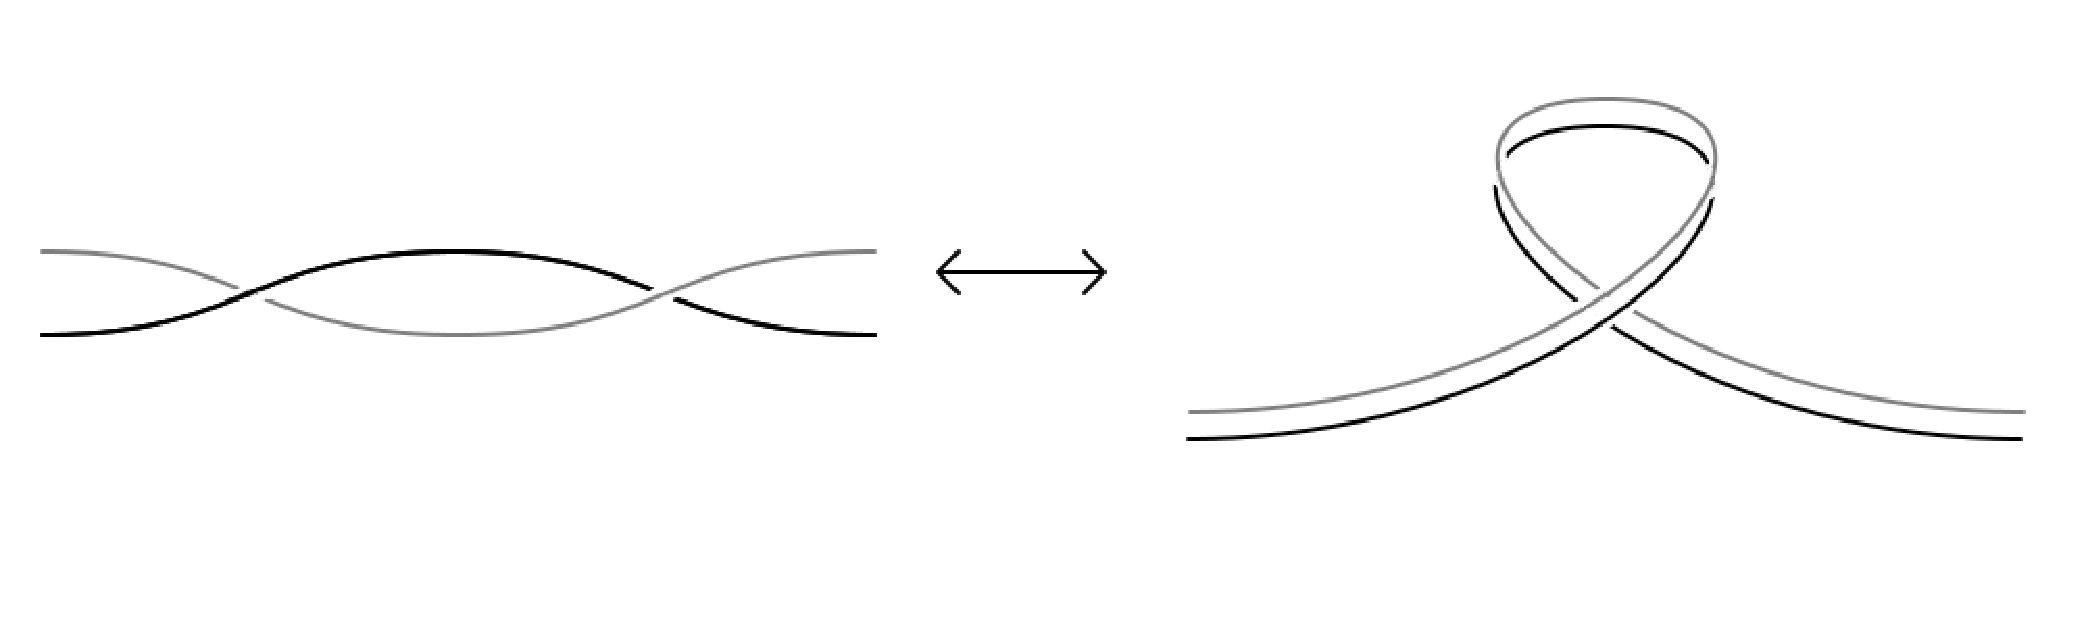
\includegraphics[width=8cm]{twistToBlackboard}
	\caption{Straightening a twist of the framing}
	\label{twistToBlackboard.fig}
\end{figure}

Thus we can specify a virtual framed isotopy class by giving a virtual topological knot whose blackboard framing is contained in that virtual framed isotopy class.  

\subsubsection{The flat projection of a virtual blackboard framed knot}
To prove Proposition $\ref{meven}$ we use an invariant that is defined on the flat diagram of a blackboard framed virtual framed knot.  As noted above a blackboard framed virtual knot may be given by a virtual topological knot $(F, K, l)$.  The flat projection of a blackboard framed knot is the immersed curve $(F, K)$ on $F$ obtained by forgetting the cooriented line field of $(F, K, l)$.

If two blackboard framed knots in the spherical cotangent bundle of the same surface are framed homotopic then their flat projections are related by a sequence of moves in Figure \ref{flatBlackboardFrontMoves.fig}.

\begin{figure}[htbp]
	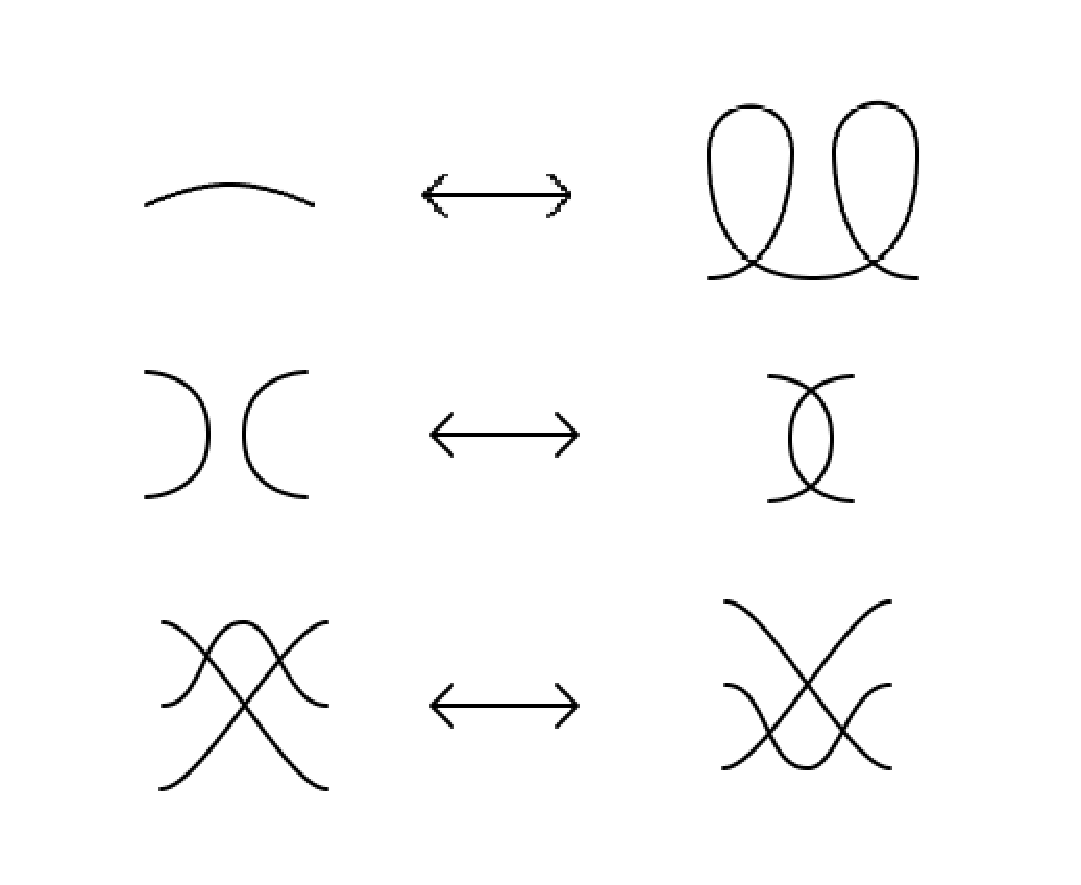
\includegraphics[width=8cm]{flatBlackboardFrontMoves}
	\caption{Moves for flat virtual blackboard framed knot projections}
	\label{flatBlackboardFrontMoves.fig}
\end{figure}

Thus if two blackboard framed virtual knots $(F,K, l)$ and $(F',K',l')$ are virtually framed homotopic then there exists a sequence of moves in Figure \ref{flatBlackboardFrontMoves.fig}, in addition to stabilization and destabilization of the surface that takes the flat projection of $(F, K, l)$ to that of $(F', K', l')$.


\subsection{Virtual Legendrian Isotopy}\label{defvirtlegiso}
Let $\bar{K}$ be a Legendrian knot in $ST^*F$ in general position.  Then $\bar{K}$ projects to a cooriented wavefront $K$ on $F$.  Furthermore, two Legendrian knots $\bar{K}_1$ and $\bar{K}_2$ are Legendrian isotopic in $ST^*F$ if and only if their wavefronts $K_1$ and $K_2$ on $F$ are related by a sequence of the moves in Figure \ref{wavefrontmoves.fig}, excluding the dangerous self-tangency move.  


Put $(F_1, K_1) \sim_l (F_2, K_2)$ if there exists a compact oriented surface $F_3$ and orientation preserving embeddings $\phi_1: F_1\rightarrow F_3$ and $\phi_2: F_2\rightarrow F_3$ such that $\phi_1(K_1)$ and $\phi_2(K_2)$ are related by a sequence of moves for wavefronts on $F_3$, or equivalently, if $\overline{\phi_1(K_1)}$ and $\overline{\phi_1(K_1)}$ are Legendrian isotopic in $ST^*F_3$.  

We say $(F,K)$ and $(F',K')$ are {\it virtually Legendrian isotopic} if there exists a sequence of pairs satisfying  $$(F,K)=(F_1,K_1)\sim_l (F_2, K_2)\sim_l \dots \sim_l (F_m,K_m)=(F',K').$$

\begin{rem} If in this definition we allowed dangerous tangency moves as well then we would have the definition of a virtual Legendrian homotopy.
\end{rem}

\begin{rem} A virtual Legendrian knot in a cooriented contact structure has a natural framing, at each point given by the unit vector in the normal bundle to the velocity vector of the knot on which the coorienting one form evaluates to one.
\end{rem}

%\begin{rem}  It is straightforward to check that an orientation preserving embedding $\phi:F\rightarrow F'$ induces a contactomorphism from $ST^*F$ to $ST^*F'$. Indeed given a contact plane $C=\pi_*^{-1}(l_\omega)$ at $\omega_p \in ST^*F$, we consider its image under $\phi$  
	
	
%	Indeed, given an orientation preserving embedding $\phi : F \rightarrow F'$ we would like $\phi^{-1*} : ST^*F \rightarrow ST^*F'$ to take a Legendrian knot to a Legendrian knot.  Let $\pi:ST^*F\rightarrow F$ and $\pi':ST^*F'\rightarrow F'$ be the natural projections.  Also note that the standard contact plane at  $p \in ST^*F$ is denoted by $\ell_p$ and is defined to be $\ell_p = \pi_*^{-1}(ker(p)) \subset TST^*F$.  So if $X\in \ell_p$ then we have that $p(\pi_*(X))=0$.  Now we want $(\phi^{-1*})_*(X)\in \ell_{\phi^{-1*}(p)} \Leftrightarrow \phi^{-1*}(p)(\pi'_*(\phi^{-1*})_*(X))=0$.  Unravelling this we have:
%\begin{align*}
%	\phi^{-1}*(p)(\pi'_*(\phi^{-1*})_*(X)) &= \phi^{-1*}(p)(\phi_*\pi_*(X))\\
%			&= p(\phi^{-1}_*\phi_*\pi_*(X))\\
%			&= p(\pi_*(X))\\
%			&= 0
%\end{align*}
%Thus the natural contact plane is taken to the natural contact plane, and hence Legendrian knots are taken to Legendrian knots.

%\end{rem}

\section{Flat Framed Virtual Knot Diagrams}
In this section we give formulations of the theory of virtual framed knots in $ST^*F$ and virtual Legendrian knots in terms of planar diagrams.
\subsection{Flat Virtual Framed Knot Diagram}
Given a virtual knot with a blackboard framing, $(F, \bar{K}, l)$ we associate to it a planar flat virtual framed knot diagram.  This is obtained first by forgetting the framing and cooriented line field, leaving a generic immersed curve $K$ on the surface $F$, denoted $(F, K)$. Then we construct the Gauss diagram, or in Turaev's language \cite{Turaev}, the virtual string, associated to this curve.  This virtual string describes a flat virtual knot diagram in the plane, which is unique up to the detour move (i.e., any combination of purely virtual moves).

%DONE: THERE IS A MISSING MOVE IN FIGURE 8!!!!!!!!!!!!!!!!!!!!!!!!!!!!!!!
%TODO: CLEAN UP CIRCLES ON LAST MOVE

If two virtual framed knots are virtual framed homotopic then their planar flat virtual diagrams are related by a sequence of moves in Figure \ref{flatDiagramMoves.fig}.

\begin{figure}[htbp]
	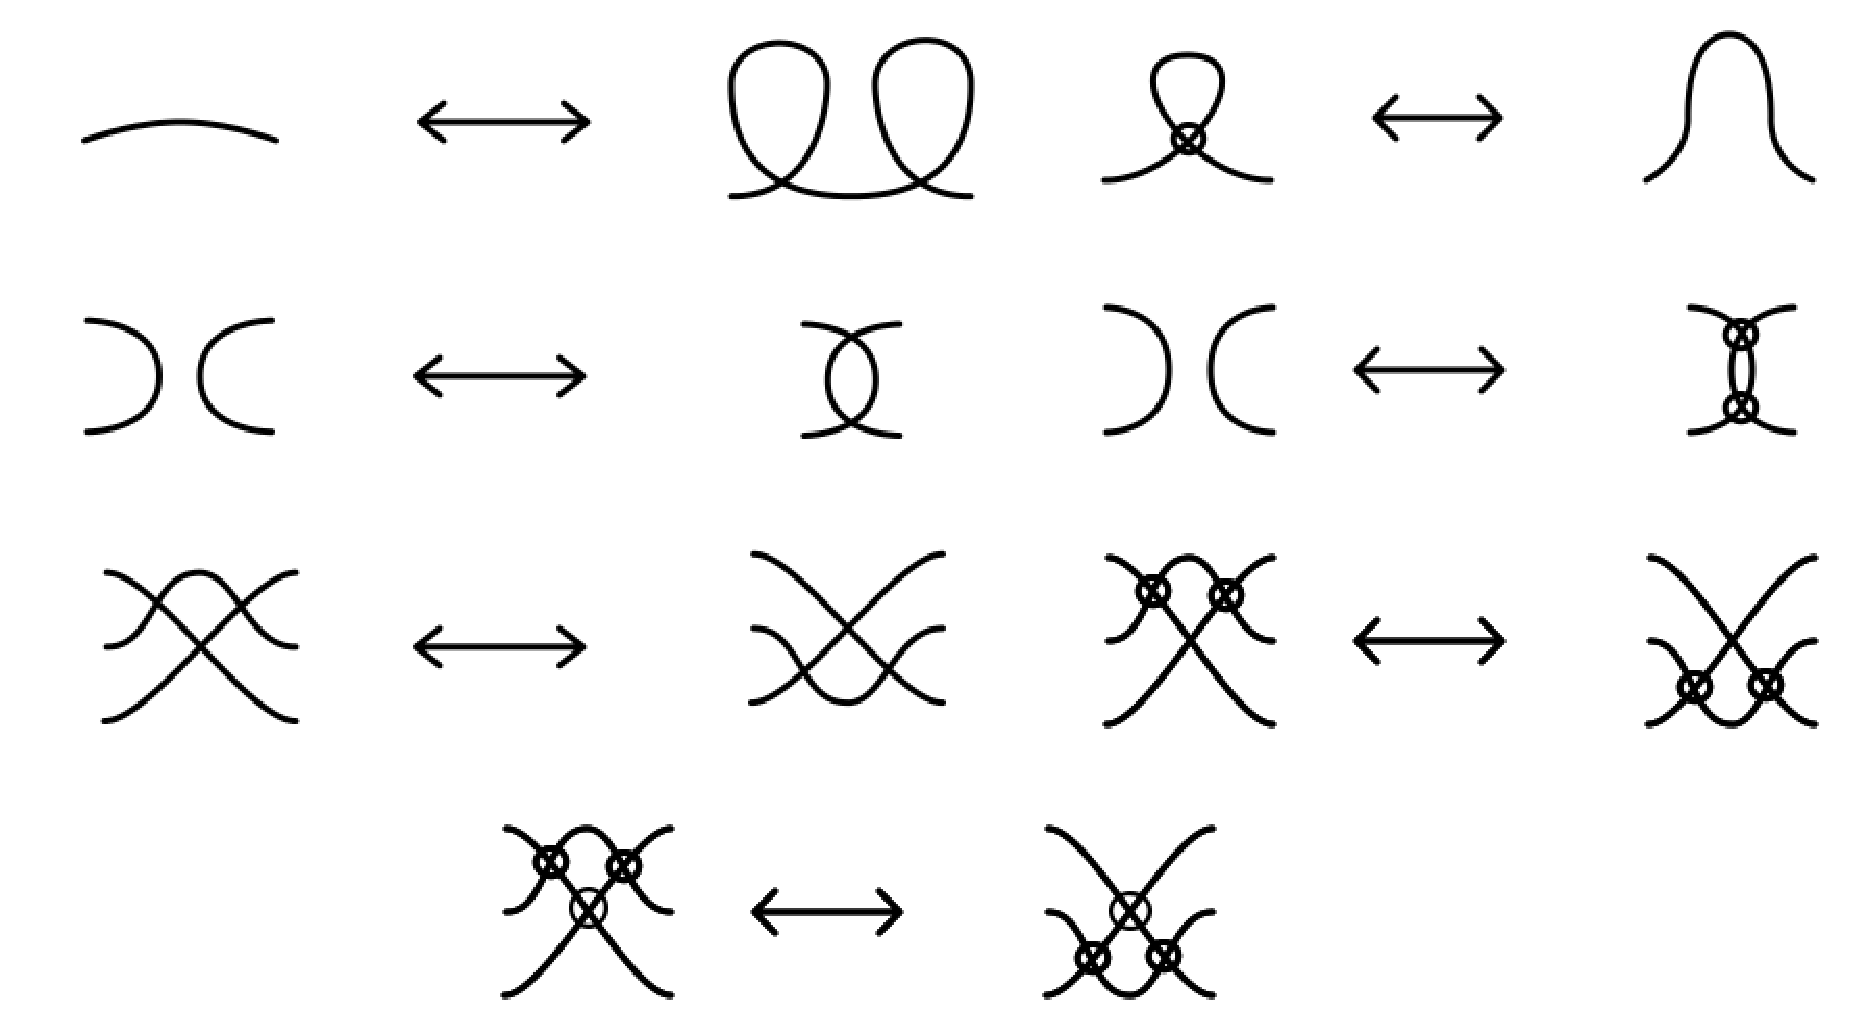
\includegraphics[width=12cm]{flatDiagramMoves}
	\caption{Moves for flat virtual framed knot diagrams}
	\label{flatDiagramMoves.fig}
\end{figure}

%\textcolor{blue}{Move twist of vector field through double point\\
%Cancel opposite twists of vector field\\
%Cancel certain pairs of kinks depending on $l$ at the crossing points-think more about precise def later\\
%R2, R3\\
%All flat moves} 
\subsection{Virtual Front Diagrams}
\section{Equivalent Definitions of Virtual Legendrian Isotopy}
 Let $\mathcal{LGD}$ be the set of Legendrian Gauss diagrams and let $\sim_{lgd}$ be the equivalence relation generated by Gauss diagram moves.  Let $LGD=\mathcal{LGD}/ \sim_{lgd}$.  

Let $\mathcal{VLD}$ be the set of virtual Legendrian knot diagrams.  Let $\sim_{vld}$ be the equivalence relation generated by virtual Legendrian knot diagram moves.  Put $VLD=\mathcal{VLD}/\sim_{vld}$.

The theory of Legendrian Gauss diagrams up to Gauss diagram moves is equivalent to the theory of virtual Legendrian knot diagrams up to virtual wavefront moves.

\begin{thm}  The map $g: \mathcal{VLD}\rightarrow \mathcal{LGD}$ given by associating a (unique) Legendrian Gauss diagram to a virtual Legendrian knot diagram induces a bijection $g_\sim :VLD\rightarrow LGD$.
 \end{thm}
\pp  
First we verify that $g_\sim$ is well-defined.  Indeed, the Legendrian Guass diagrams of two equivalent virtual Legendrian knot diagrams differ by Gauss diagram moves, as moves involving virtual crossings do not affect the Gauss diagram.  

The map $g_\sim$ is clearly surjective, as any Legendrian Gauss diagram gives rise to a virtual Legendrian knot diagram.  One simply draws all cusps and crossings present in the Legendrian Gauss diagram in the plane, and connects such cusps and crossings by arcs, creating virtual crossings where these arcs cross.

It remains to check that $g_\sim$ is injective.  Suppose we have two virtual Legendrian knot diagrams $D_1$ and $D_2$ with the same Gauss diagram.  We will show that $D_1$ and $D_2$ are related by virtual Legendrian knot diagram moves.  We first change $D_2$ by a regular isotopy so that a small neighborhood of each of its cusps and double points coincides with a small neighborhood of each corresponding cusp and double point of $D_1$.  The resulting diagrams differ only in how the cusps and double points are connected by arcs.  To move an arc $a_2$ of $D_2$ so that it coincides with the corresponding arc $a_1$ of $D_1$, we move $a_2$ by a fixed endpoint homotopy, such that any crossings created during that homotopy are virtual.  This move is known as the {\it detour move}, and is simply a sequence of the moves pictured in Figure \ref{virtualwavefrontmoves.fig}. 
\qed

Now let $\mathcal{SFD}$ be the set of all front diagrams on orientable surfaces, i.e., all pairs $(F,D)$ where $F$  is an oriented surface and $D$ is a cooriented wavefront on $F$.  Let $\sim_{sfd}$ be the equivalence relation generated by the relation $\sim_l$ defined in Subsection \ref{defvirtlegiso}, and let $SFD=\mathcal{SFD}/\sim_{sfd}$.  In other words, $SFD$ consists of pairs $(F,D)$ of oriented surfaces $F$ with cooriented wavefront diagrams $D$ on $F$ considered up to wavefront moves and stabilization and destabilization of the surface $F$.

Next we show that the theory of Legendrian Gauss diagrams up to Gauss diagram moves is equivalent to the theory of fronts on surfaces up to wavefront moves.
\begin{thm} The map $h: \mathcal{SFD}\rightarrow \mathcal{LGD}$ that assigns a Legendrian Gauss diagram to a wavefront on an oriented surface induces a bijection $h_\sim : SFD \rightarrow LGD$.
\end{thm}
\pp  First we check that $h_\sim$ is well-defined.  That is, suppose we have two pairs $(F,D)$ and $(F', D')$, such that for some sequence of pairs $\{(F_i,D_i)\}_{i=1}^n$, we have
$$(F,D)=(F_1,D_1)\sim_l (F_2,D_2)\sim_l \dots (F_n, D_n)=(F',D').$$
We need to check that $(F,D)$ and $(F',D')$ have equivalent Legendrian Gauss diagrams, but since stabilization and destabilization do not affect the Legendrian Gauss diagram of a wavefront on a surface, this is clear.

Next we verify that $h_\sim$ is surjective.  To do this, we explain how to construct a wavefront diagram on a surface given a Legendrian Gauss diagram.   First we build the disk-band surface realizing the underlying flat virtual knot of the wavefront.  Then we add signs and cusps as given by the markings on the Legendrian Gauss diagram.

\qed

\section{Virtual Versions of the Classical Invariants}\label{classical.sec}

In this section we define the Maslov and Bennequin numbers for virtual Legendrian knots.

\subsection{Maslov number.}   The virtual Maslov number $\mu(K_v)$ where $K_v$ is a planar virtual front diagram, is defined to be the number of positive cusps minus the number of negative cusps; see Figure \ref{cusps.fig}.  Clearly, if $K_v$ corresponds to the front $(F,K)$ on a surface then $\mu(K_v)$ is equal to the (non-virtual) Maslov number of the front $K$ on $F$.

A {\it positive (respectively negative) stabilization} of the virtual Legendrian knot $K$ is obtained by inserting a pair of positive (respectively negative) cusps at any point along $K$.  Let $K^{n_1,n_2}$ denote the virtual Legendrian knot obtained from $K$ by applying $n_1$ positive stabilizations and $n_2$ negative stabilizations.  

\begin{prop}\label{propposnegstab} The virtual Legendrian knot $K$ is virtual Legendrian homotopic to $K^{n,n}$ for any positive integer $n$.
\end{prop}
\pp One can add a pair of positive cusps and a pair of negative cusps using a Legendrian homotopy; see Figure \ref{homotopyposnegstabilization}.  This sequence of moves is due to Fuchs and Tabachnikov \cite{f&t}.  This Legendrian homotopy is also a virtual Legendrian homotopy.
\begin{figure}[htbp]\label{homotopyposnegstabilization}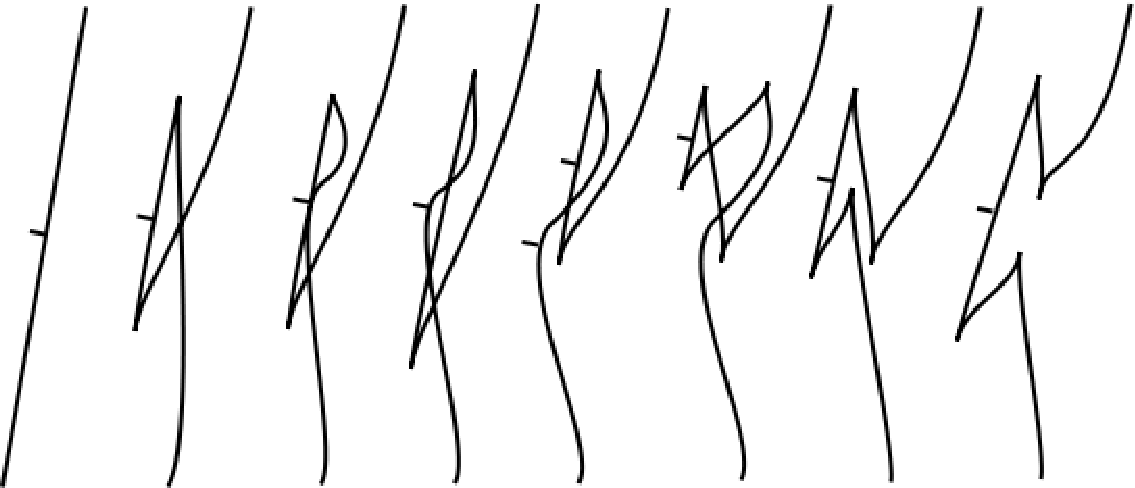
\includegraphics[width=9cm]{homotopyposnegstabilization}
	\caption{Adding a pair of negative cusps and a pair of positive cusps via a (virtual) Legendrian homotopy.}
\end{figure}
\qed

\begin{thm} Two virtual Legendrian knots are virtual Legendrian homotopic if and only if they have the same virtual Maslov number and are homotopic as virtual knots.
\end{thm}
\pp One can verify that the virtual Maslov number is an invariant of virtual Legendrian homotopy by checking its invariance under all virtual wavefront moves, as well as the dangerous tangency move.  Hence two virtual Legendrian homotopic virtual Legendrian knots have the same virtual Maslov number and (clearly) are homotopic as virtual knots.

Now suppose that $K$ and $L$ are Legendrian knots with the same virtual Maslov number that are homotopic as virtual knots.  We will show below that the assumption that $K$ and $L$ are homotopic implies that for sufficiently large positive integers $n_1$ and $n_2$, there exist integers $n_3$ and $n_4$ such that $K^{n_1, n_2}$ is virtual Legendrian homotopic to $L^{n_3,n_4}$.  In particular, this will be true for some $p=n_1=n_2$ large enough.  Then, since $K$ and $K^{p,p}$ are virtual Legendrian homotopic by Proposition \ref{propposnegstab}, and for suitable $n_3$ and $n_4$, $K^{p,p}$ and $L^{n_3,n_4}$ are virtual Legendrian homotopic, we have that $\mu(L)=\mu(K)=\mu(K^{p,p})=\mu(L^{n_3,n_4})$.  Then $\mu(L)=\mu(L^{n_3,n_4})$ implies $n_3=n_4$.  Put $q=n_3=n_4$.  Again by Proposition \ref{propposnegstab}, $L$ and $L^{q,q}$ are virtual Legendrian homotopic. Hence $K$ and $L$ are virtual Legendrian homotopic.

It remains to show that if $K$ and $L$ are homotopic then for sufficiently large positive integers $n_1$ and $n_2$, there exist integers $n_3$ and $n_4$ such that $K^{n_1, n_2}$ is virtual Legendrian homotopic to $L^{n_3,n_4}$.

Hence we let $K$ be a Legendrian knot in $ST^*F$ with its canonical contact structure, $L$ be a Legendrian knot in $ST^*F'$ with its canonical contact structure, and we have a sequence of pairs
$$(K,F)=(K_1,F_1),(K_2,F_2),\dots,(K_n,F_n)=(L,F')$$
of curves $K_i$ in $ST^*F_i$ such that the cooriented line fields $\bar{K_i}$ on $F_i$ and $\bar{K_{i+1}}$ on $F_{i+i}$ lifting to $K_i$ and $K_{i+1}$ respectively can be realized as homotopic cooriented line fields on a third surface $G_i$ (meaning their lifts are homotopic in $ST^*G_i$).  

On each surface $G_i$, this homotopy looks locally like a sequence of Reidemeister moves and crossing changes. We show how to imitate this virtual homotopy by a virtual Legendrian homotopy by replacing topological Reidemeister moves with Legendrian Reidemeister moves, and by replacing topological crossing changes with Legendrian crossing changes.
 
The argument is now local, so we simply consider the case where $K$ and $L$ are homotopic as Legendrian knots in $ST^*F$ for a fixed surface $F$.  Furthermore we assume for now that the homotopy between $K$ and $L$ is contained in a single Darboux chart, so that $K$ and $L$ are Legendrian knots in the standard contact $\mathbb{R}^3$.  We consider the topological knot projections of $K$ and $L$ to the $xz$-plane.  Because $K$ and $L$ are homotopic, their topological projections are related by a sequence of Reidemeister moves of Types 1-3 and crossing changes; see Figure \ref{crossingchange.fig}.

Fuchs and Tabachnikov \cite{f&t} proved that if $K$ and $L$ are topologically isotopic Legendrian knots in the standard contact $\mathbb{R}^3$, then  for sufficiently large $n_1$ and $n_2$, there exist  $n_3$ and $n_4$ such that $K^{n_1, n_2}$ is Legendrian isotopic to $L^{n_3, n_4}$.  We prove the same statement, replacing isotopy with homotopy, and imitate their proof.  Let $\kappa$ and $\lambda$ be the front projections of $K$ and $L$. First we know $\kappa$ and $\lambda$ are related by a topological isotopy $K_t$ with projection $\kappa_t$, such that $K_0=K$, $K_1=L$, and for some $0=t_0<t_1< t_2 < \dots <t_n=1 \in [0,1]$, $\kappa_i=\kappa_{t_i}$ and $\kappa_{i_1}=\kappa_{t_{i+1}}$ are related by a single topological Reidemeister move, topological crossing change (see Figure \ref{crossingchange.fig}), or a passage through a vertical tangency (an ambient isotopy during which a strand without a vertical tangency passes through a vertical tangency, and after which two new vertical tangencies appear locally).

Next convert each topological knot diagram $\kappa_i$ into a front diagram by replacing vertical tangencies with cusps, and correcting ``wrong crossings" as in Fuchs and Tabachnikov \cite{f&t}, see Figure \ref{wrongcrossing.fig}.  These operations clearly do not affect the topological type of the knot.

Fuchs and Tabachnikov then show how to replace topological Reidemeister moves and passages through vertical tangencies with Legendrian versions of these moves, possibly after adding extra positive or negative cusp pairs.  It remains to show that we can do the same for topological crossing changes.  This is shown in Figure \ref{legendriancrossingchange.fig}.
\begin{figure}[htbp]\label{crossingchange.fig}
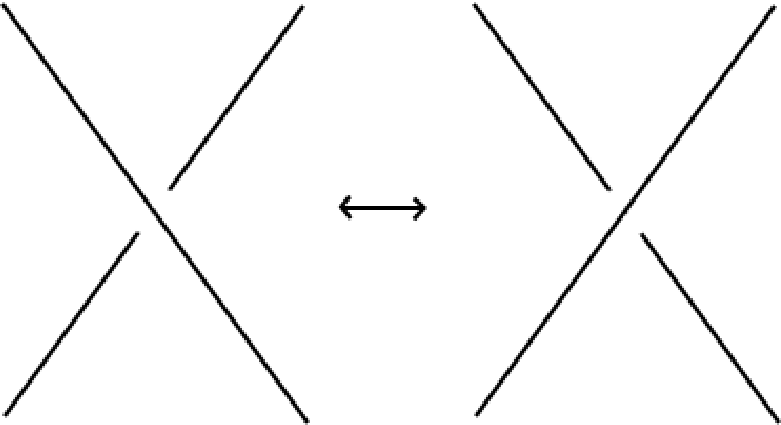
\includegraphics[width=3cm]{crossingchange}
\caption{A crossing change.}
\end{figure}
\begin{figure}[htbp]\label{wrongcrossing.fig}
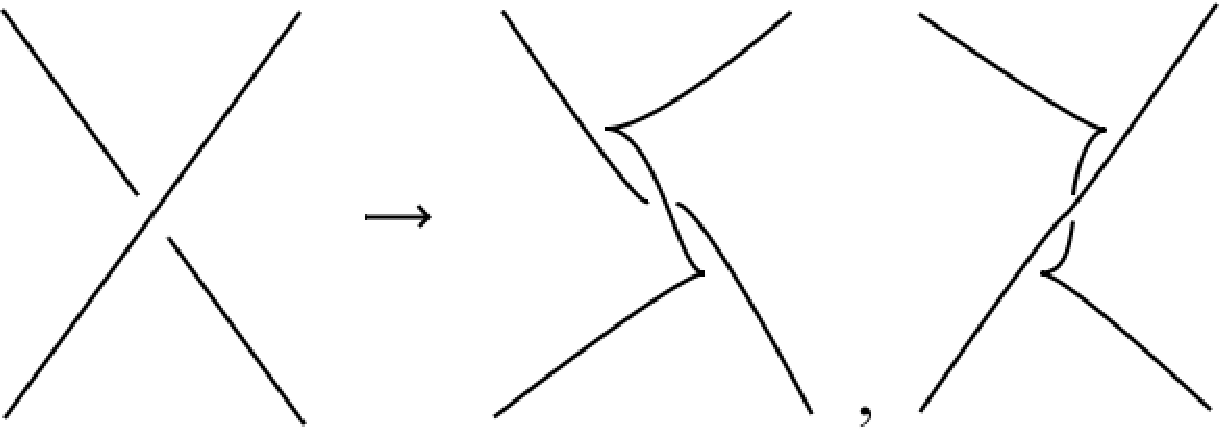
\includegraphics[width=6cm]{wrongcrossingtofrontdiagram}
\caption{Converting a ``wrong crossing'' in a topological knot diagram to a front projection of a Legendrian knot in standard contact $\mathbb{R}^3$.}
\end{figure}
\begin{figure}[htbp]\label{legendriancrossingchange.fig}
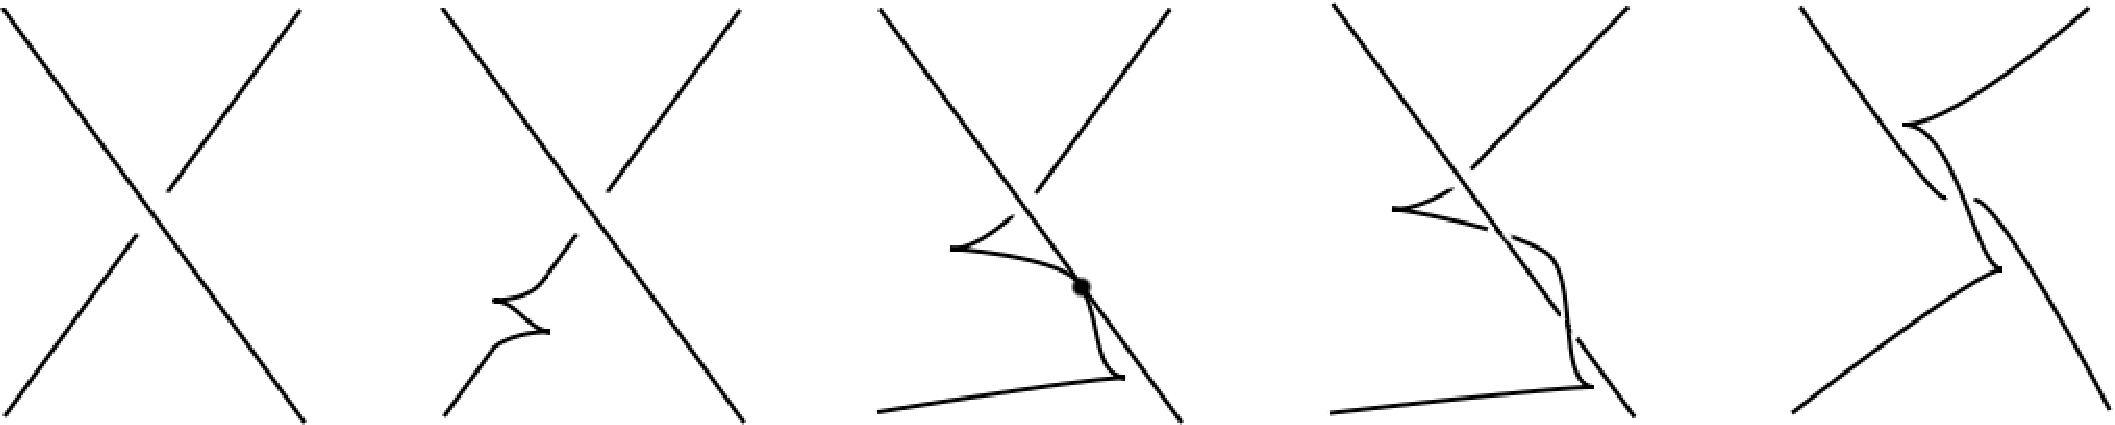
\includegraphics[width=9cm]{legendriancrossingchange}
\caption{After adding cusp pairs, we can replace a topological crossing change with a Legendrian crossing change.}
\end{figure}
\qed

%\subsection{The Bennequin Number.}  For ordinary (non-virtual) Legendrian knots in the contact manifold $(M,C)$, the Bennequin number is defined to be the self-linking number of a zerohomologous Legendrian knot.  For wavefronts on a surface, the Bennequin number differs from Arnold's $J^+$ by a constant CITE, so we may use Arnold's $J^+$ invariant as a substitution for the Bennequin number of a Legendrian knot in the spherical cotangent bundle of a surface.

% Polyak \cite{Polyak} found a formula for the $J^+$ invariant of a planar front in terms of its Gauss diagram.  



\section{Vassiliev Invariants}
In this section we define finite order Vassiliev invariants for virtual Legendrian, framed and topological knots. For the rest of the paper let $\mathcal{A}$ be an abelian group.

A self-intersection point of an immersed curve is called transverse if the two velocity vectors to the curve at that point are linearly independent.  An $n$-singular virtual Legendrian (resp. framed, topological) knot is a virtual Legendrian (resp. framed, topological) knot with $n$ transverse self-intersection points.

In an oriented $3$-manifold a transverse self-intersection point of an immersed curve can be resolved in two ways.  We call the resolution positive if the velocity vector to one strand, the velocity vector to the second strand and the vector from the second to the first strand form a positive $3$-frame.  Otherwise the intersection is called negative.  Given an immersed curve with $(n+1)$ transverse self intersection points there are $2^{n+1}$ possible ways to resolve these intersection points. We define the {\it sign of a resolution} to be the product of the signs of the resolutions of all of the individual double points. 

An $\mathcal{A}$-valued virtual Legendrian (resp. framed, topological) knot invariant is a function from the set of virtual Legendrian (resp. framed, topological) isotopy classes to $\mathcal{A}$.

A Vassiliev invariant of virtual Legendrian (resp. framed, topological) order $\leq n$ is an $\mathcal{A}$-valued virtual Legendrian (resp. framed, topological) knot invariant that vanishes on the signed sum of the $2^{n+1}$ resolutions of any $(n+1)$-singular virtual Legendrian (resp. framed, toplogical) knot.
 
\section{Construction of the Isomorphism}
When studying Vassiliev invariants of virtual Legendrian knots, we consider invariants of knots from a single connected component of the space of virtual Legendrian curves (i.e., a single virtual Legendrian homotopy class).  This is because virtual Legendrian knots that are not virtually Legendrian homotopic have no chance of being virtually Legendrian isotopic.  Similarly, when studying Vassiliev invariants of virtual framed knots, we consider invariants of knots from a single connected component of the space of framed curves.

In this paper we will show that Vassiliev invariants cannot be used to distinguish virtual Legendrian knots in the same virtual Legendrian homotopy class that are isotopic as framed virtual knots.  First we prove the following seemingly weaker statement:

\begin{thm} \label{statementA}
Let $x\in \mathcal{V}_n^\mathcal{L}$.  Suppose $(F_1, K_1)$ and $(F_2, K_2)$ are two virtual Legendrian knots in $ \mathcal{L}$, such that $(F_1, K_1)$ is virtual framed isotopic to $(F_2, K_2)$.   Then $x(F_1, K_1) = x(F_2, K_2)$.
\end{thm}

Using this theorem we are then able to prove the following stronger statement:

\begin{thm} \label{statementB}
Let $\mathcal{F}$ be a connected component of the space of virtual framed curves and $\mathcal{L}\subset\mathcal{F}$ be a connected component of the space of virtual Legendrian curves contained in $\mathcal{F}$.  Let $\mathcal{A}$ be an abelian group and $\mathcal{V}_n^\mathcal{F}$ be the group of $\mathcal{A}$ valued Vassiliev invariants on $\mathcal{F}$ of order $\leq n$.  Define $\mathcal{V}_n^\mathcal{L}$ likewise.  Then the restriction map $\phi:\mathcal{V}_n^{F}\rightarrow\mathcal{V}_n^\mathcal{L}$ is an isomorphism.
\end{thm}

% \textcolor{red}{DELETE The most obvious idea for constructing this inverse would be to simply extend $x\in\mathcal{V}_n^\mathcal{L}$ to $\mathcal{F}$ by deforming the argument of $x$ (which started as a virtual framed knot) by a virtual framed isotopy to a virtual Legendrian knot.  It is not clear that this will be well defined though, since there may be more that one virtual Legendrian isotopy class in the same virtual framed isotopy class.. But the following result shows that it is actually well defined.} In order to construct an inverse we show Vassiliev invariants cannot distinguish virtually framed isotopic Legendrian knots that are in the same component of the space of virtual Legendrian curves:


It is clear that Theorem \ref{statementB} implies Theorem \ref{statementA}.  In this section we will show that Theorem \ref{statementA} implies Theorem \ref{statementB}.  We will prove Theorem \ref{statementA} in a later section.

Now we outline the construction of an inverse, $\psi$, to the map $\phi$ defined above.  If the framed isotopy class of $(F,K)$ contains a Legendrian representative $(F_l,K_l)$ then we define $\psi(x)(F,K)=x(F_l,K_l)$.  By Theorem \ref{statementA}, this is well-defined. If every virtual framed isotopy class were realizable by a virtual Legendrian knot, then the existence of $\psi$ would follow immediately from Theorem \ref{statementA}.  The Bennequin inequality tells us that not every (non-virtual) framed isotopy class is realizable by a Legendrian knot in, for example, $\mathbb{R}^3$ with the standard contact structure.  However, no Bennequin inequality is known for virtual Legendrian knots.  Therefore it is could be that every virtual framed isotopy class is realizable by a virtual Legendrian knot; this question is currently open.



%\textcolor{red}{DELETE Thus we have that if two virtual Legendrian knots are virtual framed isotopic then a Vasilliev invariant of virtual Legendrian knots must take the same value on both of them.  This hints that it might be possible to simply extend a Vasilliev invariant of virtual Legendrian knots to one of virtual framed knots. ??  However, we would still need to define $\psi$ on virtual framed isotopy classes that contain no virtual Legendrian knot. }

%First we characterize part of the connected component containing a given virtual framed knot in Proposition \ref{conncomp}, and describe which isotopy classes in that component contain virtual Legendrian knots in Proposition \ref{prop2i}.  


% Given a framed knot $\bar{K}$ in $ST^*F$, we can count the number of twists of the framing of $\bar{K}$, with respect to a certain blackboard framing.  Recall that $K$ is the projection of $\bar{K}$ to $F$.  Consider the torus $T_K$ over $K$ in $ST^*F$, which is simply the union of the fibers over $K$.  Then $\bar{K}$ is a curve on $T_K$.  Now shift $\bar{K}$ slightly in the direction of its framing to get a curve $\bar{K}_f$.  Consider a thin tubular neighborhood of $\bar{K}$ such that $\bar{K}_f$ lies on the (torus) boundary of that neighborhood, which we denote by $T_f$.  Now $T_f$ intersects $T_K$ in two curves $C_1$ and $C_2$ (assume that if one goes from $C_1$ to $C_2$ along the fiber in the direction of its orientation, this is shorter than going along the fiber from $C_2$ to $C_1$).  Consider the minimal intersection number of $C_1$ and $\bar{K}_f$ as curves on $T_f$.  This number is called the {\it number of twists of the framing $\#\bar{K}$ of $\bar{K}$} (if we used $C_2$ instead the answer would be multiplied by $-1$).  Each intersection of $\bar{K}_f$ with $T_K$ appears on $F$ as an intersection point of $K$ and $K_f$, so one can compute this number combinatorially from the knot diagram.  
% 
% For framed knots $K_1$ and $K_2$ that coincide pointwise as embeddings but not necessarily as framed knots, we put $m(K_1,K_2)=\#K_1-\#K_2$, and call this the {\it relative number of framings of $K_1$ and $K_2$}.  If $m(K_1,K_2)=i$, we write $K_2=K_1^i$.


Given two virtual framed knots $K_1=(F,K_l^{\nu_1})$ and $K_2=(F,K_2^{\nu_2})$ that coincide as pointwise embeddings in the same spherical cotangent bundle $ST^*F$, we can measure the relative number of twists of their framings as follows.  The frame consisting of $\bar{K}'(t) \times \nu_1(t)$ and the vector ${\nu_1}(t)$, gives a trivialization of the normal bundle of $\bar{K}$.  Define $m(K_1,K_2)$ to be the total number of rotations of the projection of $\nu_2$ with respect to this trivialization.

% Note that there is an analogue of the blackboard framing of a knot in $ST^*F$, where all framing vectors point in the positive direction of the fiber.  The number of framings of a knot is just the number of framings relative to the same knot with the ``blackboard'' framing.

In Proposition \ref{meven} we use $m$ to characterize the connected components of the space of virtual framed knots.

For the proof of Proposition \ref{meven} we need the following definition.  Given a virtual framed knot $K^\nu = (F, K^\nu)$ consider one of its corresponding flat virtual framed knot diagrams in $\mathbb{R}^2$.  Let $r$ be the rotation number of this curve and let $v$ be the number of virtual crossings.  Put $\rho(K^\nu) = r + v \mod{2}$.  One can check that this quantity does not change under any moves in Figure \ref{flatDiagramMoves.fig}, and thus is well-defined across all possible framed knot diagrams for a given knot. Furthermore this also shows that it is invariant under virtual framed homotopy. 

\begin{prop} \label{meven}
Let $K_1^{\nu_1} = (F, K_1^{\nu_1})$ and $K_2 = (F, K_2^{\nu_2})$ be virtual framed knots (resp. singular virtual framed knots with n transverse double points) that coincide pointwise as embeddings (resp. immersons) in $ST^*F$.  Then $K_1^{\nu_1}$ and $K_2^{\nu_2})$ are virtual framed homotopic if and only if $m( K_1^{\nu_1}, K_2^{\nu_2})$ is even.
\end{prop}
\pp If $m( K_1^{\nu_1}, K_2^{\nu_2})$ is even, then $K_1^{\nu_1}$ and $K_2^{\nu_2}$ are homotopic as framed knots in $ST^*F$ because one can pass through a small kink to change $m$ by two.

Now suppose $m( K_1^{\nu_1}, K_2^{\nu_2})$ is odd.  Since $m$ is odd we must have that $\rho(K_1) \neq \rho(K_2)$.  Thus $K_1^{\nu_1}$ cannot be virtual framed homotopic to $K_2^{\nu_2}$.

\qed

Suppose that $K=(F,K,l,W)$ and $K'=(F,K,l,W')$ coincide as smooth embeddings, and $m(K,K')=i$.  Then we write $K'=K^i$.

%This characterization is a generalization of that found in Chernov \cite{Chernov} and our definition of $m(\dot, \dot)$ is the same as his.  This invariant is constructed to be a generalization of the self-linking number of framed knots.  Namely:
%\textcolor{red}{get rid of vector fields; fix spelling of Vassiliev}
%\begin{defin}\footnote{is this well defined?}
%Let $(F_1, K_1, V_1, W_1)$ and $(F_1, K_2, V_2, W_2)$ be two virtual framed knots whose liftings coincide pointwise as embeddings of $S^1$ (i.e. $K_1 = K_2$ and $V_1 = V_2$).  Let $(F_1, K_1', V_1', W_1')$ be the knots obtained by shifting $\overline{K_1}$ slightly along its framing.  Now $\overline{K_1}$ and $\overline{K_1'}$ bound a thin strip.  Define $m((F_1, K_1), (F_2, K_2))$ to be the sum of the signed intersections of a small shift of $\overline{K_2}$ along its framing with this strip.
%\end{defin}

We want to prove that Theorem \ref{statementB} implies that the inverse $\psi$ described above exists. In \cite{Chernov} it is  shown that an analogue of Theorem \ref{statementB} for ordinary Legendrian and framed knots in most contact manifolds implies that an analogue Theorem \ref{statementA} holds, i.e., the inverse $\psi$ exists. The proof in \cite{Chernov} that $\psi$ exists is mostly local.  One can check that the same proof will work in the virtual category provided the following two propositions hold:

\begin{prop}  \label{prop2i}
Let $\mathcal{F}$ be a connected component in the space of virtual framed curves (resp. singular curve), and $\mathcal{L}\subset\mathcal{F}$ be a connected component in the space of virtual Legendrian curves (resp. singular curves).  Let $K\in\mathcal{F}$ be a virtual framed knot (resp. singular knot). Then there exists $i\in\mathbb{Z}$ and a virtual Legendrian knot (resp. singular knot) $K'\in \mathcal{L}$ such that $K'\in [K^{2i}]_f$.  Furthermore if there exists a virtual Legendrian knot (resp. singular knot) $K'\in \mathcal{L}$ such that $[K']_f = [K]_f$ then there exists a virtual Legendrian knot (resp. singular knot) $K''\in\mathcal{L}$ such that $[K'']_f = [K^{-2}]_f$.
\end{prop}
\pp In \cite{Chernov} it is shown that for some $i \in \mathbb{Z}$, there exists a Legendrian knot $L$ in the ordinary (non-virtual) framed isotopy class of $K^{2i}$.   Take $K'=L$.  Similarly, it is shown that if the ordinary framed isotopy class of $K$ is realizable by a Legendrian knot, then the ordinary framed isotopy class of $K^{-2}$ is realizable by a Legendrian knot $L'$.  Take $K''=L'$.
\qed
\begin{prop} \label{conncomp}  Let $\mathcal{F}$ be a connected component of the space of virtual framed curves, let $K^\nu=(F,K^\nu)\in \mathcal{F}$ and let $K_u=(F,K,l)$ be an unframed virtual knot obtained by forgetting the framing on $K^\nu$. Let $[K_u]$ be the class of virtual topological knots that contains $K_u$ and $\tilde{K}^{\nu} = (\tilde{F}, \tilde{K}^{\tilde{\nu}})\in \mathcal{F}$ be a virtual framed knot with $(\tilde{F}, \tilde{K}, \tilde{l})\in [K_u]$.  Then the virtual framed isotopy classes $[\tilde{K}]_f$ and $[K^{2i}]_f$ are equal for some $i\in\mathbb{Z}$. 
\end{prop}
\pp This follows immediately from Proposition \ref{meven}.
\qed




% \begin{prop} 
% Let $K$ be a virtual framed knot lying in the connected component $\mathcal{F}$ of the space of virtual framed knots.  Then if $K'\in\mathcal{F}$ is another virutal framed knot in $\mathcal{F}$ we must have $K'$ is virtual framed isotopic to $K^{2i}$ for some $i\in\mathbb{Z}$. 
% \end{prop}
% 
% Now that we know the structure of a connected component $\mathcal{F}$ in the space of virtual framed knots we just need to find a way to extend $x$ in a consistent manner to the isotopy classes that do not contain a virtual Legendrian knot.  
% 
% \begin{prop}
% Either every virtual framed isotopy class contains a virtual Legendrian knot, or there exists some $K\in\mathcal{F}$ such that for all $i\leq 0$ $K^{2i}$ contains a virtual Legendrian knot and for all $l>0$ $K^{2l}$ does not contain a virtual Legendrian knot.  
% \end{prop}
% 
% \textcolor{red}{make concise and delete repetitive stuff; say where the proofs can be found.}

We know how to define $\psi$ on virtual framed isotopy classes containing a virtual Legendrian knot. Let $K \in \mathcal{F}$ and $i$ be the largest integer such that $[K^{2i}]_f$ contains a virtual Legendrian knot in $\mathcal{L}$.  (If no such $i$ exists, then every $[K^{2i}]$ contains a virtual Legendrian knot, so there is no problem defining $\psi$ on all of $\mathcal{F}$.) We know how to define $\psi$ on the framed isotopy classes $[K^{2j}]_f$ for $j\leq i$.  The following definition, analogous to the definition in \cite{Chernov}, extends $\psi$ to the virtual framed isotopy classes $[K^{2j}]_f$ for $j>i$. 

\begin{defin}
Fix $K\in\mathcal{F}$ and let $j$ be the maximal integer such that $[K^{2j}]$ contains a virtual Legendrian knot in $\mathcal{L}$.  For $l>j$ define 
$$\psi(x)(K^{2l}) = \sum_{i=1}^{n+1}\left( (-1)^{i+1} \frac{(n+1)!}{i!(n+1-i)!}\psi(x)(K^{2l-2i}) \right)$$
\end{defin}

This definition extends $x$ such that it is a Vassiliev invariant of virtual framed knots of order $\leq n$ and also $\phi \circ \psi = id_{\mathcal{V}_n^\mathcal{L}}$  and $\psi \circ \phi = id_{\mathcal{V}_n^\mathcal{F}}$ as we wanted.  A directly analgous proof to this is given in \cite{Chernov}.


\section{Proof of Theorem \ref{statementA}}
Fix a connected component $\mathcal{F}$ of the space of virtual framed curves and a connected component $\mathcal{L}$ of the space of virtual Legendrian curves such that $\mathcal{L}\subset \mathcal{F}$.

In this section we will prove the following theorem:

\begin{thm} \label{samevalues}
Let $x\in \mathcal{V}_n^\mathcal{L}$.  Suppose $(F_1, K_1)$ and $(F_2, K_2)$ are two virtual Legendrian knots in $ \mathcal{L}$, such that $(F_1, K_1)$ is framed isotopic to $(F_2, K_2)$.   Then $x(F_1, K_1) = x(F_2, K_2)$.
\end{thm}

There are two types of cusps, positive (see Figure \ref{cusps.fig}).  Let $K=(F,K)$ be a virtual Legendrian knot, and let $K^{n,m}$ be the virtual Legendrian knot obtained by adding $n$ positive cusp pairs and $m$ negative cusp pairs to $K$.  A crucial tool in the proof of Theorem \ref{samevalues} is the following lemma:

\begin{lem}\label{zigzag} Let $(F_1,K_1), (F_2, K_2) \in \mathcal{F}$ be two virtual Legendrian knots. Suppose there exists $n\in \mathbb{Z}$ such that $(F_1,K_1^{n,n})$ and $(F_2,K_2^{n,n})$ are virtually Legendrian isotopic.  Let $x\in\mathcal{V}^\mathcal{F}_n$.  Then $x(F_1,K_1)=x(F_2,K_2)$.
\end{lem}

In order to use the previous lemma we must first show that the integer $n$ in Lemma \ref{zigzag} exists whenever $(F_1,K_1)$ and $(F_2,K_2)$ are in the same connected component of the space of virtual Legendrian curves and are isotopic as virtual framed knots.

To do this, we show that for $n_1,n_2$ large enough, there exists $n_3,n_4$ such that $(F_1,K_1^{n_1,n_2})$ and $(F_2,K_2^{n_3,n_4})$ are virtually Legendrian isotopic.  Then we show that we can assume that $n_1+n_2=n_3+n_4$ and $n_1-n_2=n_3-n_4$.  It will follow that $n_1=n_2=n_3=n_4$.


\begin{prop}\label{fuchstab}
Let $(F, K)$ and $(F', K')$ be virtually isotopic Legendrian knots.  Then there exist $n_1, n_2, n_3$ and $n_4$ such that $(F',K'^{n_1,n_2})$ is virtually Legendrian isotopic to $(F', K'^{n_3, n_4})$.
\end{prop}
\pp
We know that $(F_1, K_1)$ and $(F_2, K_2)$ are virtually isotopic Legendrian knots, so by definiton we a sequence of virtual knots $(F_i, K_i)$ such that: 
$$(F,K,l)=(F_1,K_1,l_1)\sim (F_2,K_2,l_2) \sim \dots \sim (F_m,K_m,l_m)=(F',K',l')$$
We will procede by induction on $m$, which is the length of this sequence.  First, if $m=2$ then this is simply the result of Fuchs and Tabachnikov as used in \cite{Chernov}.  Now, suppose the result holds for $m$ and we have the following sequence: 
$$(F,K,l)=(F_1,K_1,l_1)\sim (F_2,K_2,l_2) \sim \dots \sim (F_{m+1},K_{m+1},l_{m+1})=(F',K',l')$$
From the induction hypothesis we have $k_1,k_2, k_3$ and $k_4$ so that $(F_1,K_1^{k_1,k_2})$ is virtually Legendrian isotopic to $(F_m, K_m^{k_3, k_4})$.  Also we get $l_1, l_2, l_3$ and $l_4$ so that $(F_m,K_m^{l_1,l_2})$ is virtually Legendrian isotopic to $(F_{m+1}, K_{m+1}^{l_3, l_4})$.  For large enough $k_i, l_i$ we can freely slide the cusp pairs around using moves defined in \cite{f&t}.  So if $l_i \leq k_i$  we can just move the cusp pairs to where they are at the beginning of the final isotopy and follow it in the last step, ignoring the extra cusp pairs.  Otherwise we can set $j_i = \max\{k_i, l_i\}$.  Then by following the same isotopy as above, ignoring the extra cusp pairs, we have $(F_1,K_1^{j_1,j_2})$ is virtually Legendrian isotopic to $(F_m, K_m^{j_3, j_4})$.  But now $l_i \leq j_i$, so we can follow the final step of the isotopy and have proved the induction step.

\begin{thm}
Let $(F, K)$ and $(F', K')$ be two virtual Legendrian knots in the same virtual framed isotopy class $\mathcal{F}$, and also in the same connected component of virtual Legendrian knots $\mathcal{L}$. Then given large enough $n_1, n_2, n_3, n_4 \in \mathbb{Z}$ so that $(F, K^{n_1,n_2}) = (F',K'^{n_3, n_4})$ as virtual Legendrian knots, we have that $n_1+n_2 = n_3+n_4$.
\end{thm}

\pp
Since $(F,K)$ and $(F',K')$ are virtual framed isotopic we have a sequence of pairs:
$$(F, K) = (F_1,K_1) \sim_f (F_2, K_2) \sim_f \dots \sim_f (F_m, K_m) = (F', K').$$

More precisely we have surfaces $F_{i,i+1}$ and maps $\phi_i : F_i \rightarrow F_{i,i+1}$ and $\psi_i:F_{i+1}\rightarrow F_{i,i+1}$ such that $\phi_i(K_i)$ is framed isotopic to $\psi_i(K_{i+1})$ on $F_{i,i+1}$ via the framed isotopy $h_t^i$ for all $1\leq i < n$.  

Now, following the argument in Proposition \ref{fuchstab} we can approximate the previous framed isotopy with a Legendrian isotopy after adding sufficiently many positive and negative cusp pairs.  This yields a sequence
$$(F_1, K_1^{n_1,n_2}) = (F_1, L_1)\sim_l (F_2, L_2) \sim_l \dots \sim_l (F_m, L_m)=(F',K'^{n_3,n_4})$$

with the same surfaces $F_{i,i+1}$ and maps $\phi_i$ and $\psi_i$ as above. However, now we have a sequence of Legendrian isotopies $l_t^i:S^1\rightarrow F_{i,i+1}$ such that the image of $l_0^i$ is equal to $\phi_i(L_i)$,  and the image of $l_1^i $ is equal to $ \psi_i(L_{i+1})$.  Furthermore for all $t\in[0,1]$ we have that the image of $l_t^i$ is contained in a small torus around the image of $h_t^i$.

We can use the fact that both of these images are contained in a small torus  at each time $t$ to show that $n_1+n_2 = n_3+n_4$.

Given two framed knots $K_1=(F, K_1, l_1, L_1)$ and $K_2=(F,K_2,l_2,L_2)$ which lie in a solid torus $T$ where $T$ is embedded in $ST^*F$, we can identify $T$ with the standard torus in $\mathbb{R}^3$.  Then we define $\text{tbd}(K_1,K_2)$ to be the difference of the Thurston Bennequin numbers of the images of $K_1$ and $K_2$ under this identification.  One can check using the formula in REF $\text{tbd}(K,K^{n_1,n_2})=n_1+n_2$.

Now from the argument in \cite{Chernov} we know that $\text{tbd}$ does not change as $t$ varies.  Thus we have that $\text{tbd}(\phi_i(K_i), \phi_i(L_i)) = \text{tbd}(\psi_i(K_{i+1}), \psi_i(L_{i+1}))$.  So to finish the proof we just need to show the following: 
$$\text{tbd}(\psi_i(K_{i+1}), \psi_i(L_{i+1})) = \text{tbd}(\phi_{i+1}(K_{i+1}), \phi_{i+1}(L_{i+1}))$$
However, since $\text{tbd}$ does not depend on the identification of the torus in $F_{i,i+1}$ with the standard torus in $\mathbb{R}^3$ this equality is clear.
\qed


% However, it suffices to show that if $(F,K)\sim_f (F',K')$ then given large enough $n_1, n_2$, there exists $n_3, n_4$ such that $(F, K^{n_1,n_2}) $ and $ (F',K'^{n_3, n_4})$  are virtual Legendrian isotopic, where $n_1+n_2=n_3+n_4$.
% 
% In the proof of Proposition \ref{fuchstab}, we have a Legendrian isotopy $l_t$ of $(F_1,K_1^{n_1,n_2})$ and $(F_2, K_2^{n_3, n_4})$, and a framed isotopy $f_t$ of $(F_1,K_1)$ and $(F_2, K_2)$.  At each time $t$, let $F_t$ denote the surface such
% 
% 
% We will show that the difference between a form of Thurston Bennequin invariant of $(F_1, K_1)$ and $(F_1, K_1^{n_1, n_2})$ is constant under virtual Legendrian isotopy, and is in fact equal to $n_1+n_2$.  This will give us the desired result because we have that $(F_1, K_1^{n_1, n_2})$ is virtual Legendrian isotopic to $(F_2, K_2^{n_3, n_4})$ and thus we get $n_1+n_2 = n_3 + n_4$.
% 
% First just consider the case when this sequence is one relation long:
% $$(F, K) = (F_1,K_1) \sim_f (F_2, K_2) = (F', K')$$
% 
% By definition we then have a compact oriented surface $F_3$ and orientation preserving embeddings $\phi_1: F_1\rightarrow F_3$ and $\phi_2: F_2\rightarrow F_3$ such that $\overline{\phi_1(K_1)}$ is framed isotopic to $\overline{\phi_2(K_2)}$ in $ST^*F_3$.  Let $\mu : S^1 \times [0,1] \rightarrow ST^*F_3$ be this framed isotopy.  
% 
% Now following the previous proposition, using the virtual framed isotopy $\mu$ (which is also a virtual topological isotopy) we can find $n_1, n_2, n_3$ and $n_4$ so that $(F_1,K_1^{n_1,n_2})$ is virtually Legendrian isotopic to $(F_2, K_2^{n_3, n_4})$.  This can be done so that $\overline{\phi_1(K_1^{n_1,n_2})}$ Legendrian isotopic to $\overline{\phi_2(K_2^{n_3,n_4})}$ via $\widetilde{\mu}: S^1 \times [0,1] \rightarrow ST^*F_3$.  Note that $\widetilde{\mu}$ can be chosen so that for any $t$ we have that the Legendrian knot $\widetilde{\mu}_t:S^1\times \{t\} \rightarrow ST^*F_3$ is contained in a thin tubular neighborhood, $T_t$ of $\mu_t:S^1\times \{t\}\rightarrow ST^*F_3$ and the two knots are always topologically isotopic.
% 
% 
% 
% To define the generalization of the Thurston Bennequin invariant that we desire, take two topologically isotopic knots, $K, K'$ in a $3$-dimensional manifold with $K'$ in a thin tubular neighborhood of $K$.  We denote by $tbd(K, K')$ the difference in their Thurston Bennequin invariants under a smooth identification of the tubular neighborhood with the standard torus in $\mathbb{R}^3$.  In Chernov's paper \cite{Chernov} he showed that this difference does not depend on the identification of the tubular neighborhood with the torus and also does not change under virtual framed isotopies of the knots on a surface that keep the Legendrian knot within a thin tubular neighborhood of the topological knot.
% 
% For this definition to make sense in the category of virtual knots we first need to know that $tbd$ does not change under smooth embeddings.  
% 
% \begin{lem}
% Let $(F, K)$, $(F, K')$ be virtual knots such that $\overline{K}$ is in a thin tubular neighborhood of $\overline{K'}$ in $ST^*F$, and $\overline{K}$ is topologically isotopic to $\overline{K'}$.  Let $\phi:F\rightarrow F'$ be a smooth embedding. Then $tbd(\overline{K}, \overline{K'}) = tbd(\overline{\phi(K)}, \overline{\phi(K')})$. 
% \end{lem}
% \pp
% This follows from Chernov's observations that $tbd$ does not depend on the choice of identification of the tubular neighborhood with the torus and also does not depend on the tubular neighborhood itself.  
% 
% We can now define $tbd$ for two topologically isotopic virtual knots $(F, K)$ and $(F, K')$ with $K$ contained in a thin tubular neighborhood around $K$.  In this setup we say $tbd(F, K, K') := tbd(\overline{K}, \overline{K'})$.  We will show that $tbd(F_1, K_1, K_1^{n_1, n_2}) = tbd(F_2, K_2, K_2^{n_3, n_4})$.
% 
% From the observation above we know that $tbd$ is invariant under embeddings, and hence we have that $tbd(F_1, K_1, K_1^{n_1, n_2}) = tbd(F_3, \phi_1(K_1), \phi_1(K_1^{n_1, n_2}))$, and similarly $tbd(F_2, K_2, K_2^{n_3, n_4}) = tbd(F_3, \phi_2(K_2), \phi_2(K_2^{n_3, n_4}))$.  Now we just need to show $tbd(F_3, \phi_1(K_1), \phi_1(K_1^{n_1, n_2})) = tbd(F_3, \phi_2(K_2), \phi_2(K_2^{n_3, n_4}))$.  But it was already shown in Chernov \cite{Chernov} that in this setup $tbd$ is preserved.  Thus we have shown that $n_1 + n_2 = tbd(F_1, K_1, K_1^{n_1, n_2}) = tbd(F_2, K_2, K_2^{n_3, n_4}) = n_3 + n_4$ when the virtual framed isotopy is one relation long.
% 
% We can extend this result to an arbitrarily long virtual framed isotopy by induction.  

\begin{thm}
Let $(F, K)$ and $(F', K')$ be two virtual Legendrian knots in the same virtual framed isotopy class $\mathcal{F}$, and also in the same connected component of virtual Legendrian knots $\mathcal{L}$. Then given large enough $n_1, n_2, n_3, n_4 \in \mathbb{Z}$ so that $(F, K^{n_1,n_2}) = (F',K'^{n_3, n_4})$ as virtual Legendrian knots, we have that $n_1-n_2 = n_3-n_4$.
\end{thm}

\pp
From Proposition \ref{fuchstab} we have $n_1, n_2, n_3, n_4\in\mathbb{Z}$ so that $(F, K^{n_1,n_2}) = (F',K'^{n_3, n_4})$ as virtual Legendrian knots.  Since $K$ and $K'$ are in the same connected component of virtual Legendrian knots we have that $\mu(K)=\mu(K')$.  For the same reason we get that $\mu(K^{n_1, n_2})=\mu(K'^{n_3,n_4})$.  Finally since $K^{n_1,n_2}$ is obtained from $K$ by adding $n_1$ upward cusp pairs and $n_2$ downward cusp pairs we have $\mu(K^{n_1,n_2})-\mu(K) = n_1 - n_2$.  Similarly we have $\mu(K'^{n_3,n_4})-\mu(K')=n_3-n_4$.  So from the equalities observed above we can conclude that $n_1-n_2=n_3-n_4$
\qed

In order to prove the final theorem we need the following combinatorial lemma:

\begin{lem} \label{comboLem}
For $0\leq i < p$,
$$\sum_{k=\lceil\frac{i}{n+1}\rceil}^p (-1)^{k+1}\binom{p}{k}\binom{k(n+1)}{i} = 0$$
\end{lem}
\pp
We show this by algebraically manipulating a polynomial and comparing coeffecients.
\begin{align*}
x^p\left(\sum_{k=1}^{n+1}(-1)^k\binom{n+1}{k}x^{k-1}\right)^p &= (1-(1-x)^{n+1})^p\\
 &= \sum_{k=0}^p (-1)^k\binom{p}{k}(1-x)^{k(n+1)}\\
 &= \sum_{k=0}^p (-1)^k\binom{p}{k}\left( \sum_{j=0}^{k(n+1)}(-1)^j\binom{k(n+1)}{j}x^j \right)\\
 &= \sum_{j=0}^{p(n+1)} \left( \sum_{k=\lceil\frac{i}{n+1}\rceil}^p (-1)^{k+j}\binom{p}{k}\binom{k(n+1)}{j} \right) x^j
\end{align*}
\qed

\begin{thm}
Let $x\in \mathcal{V}_n^\mathcal{L}$, $(F_1, K_1), (F_2, K_2) \in \mathcal{L}$.  Then if there exists $p$ such that  $(F_1, K_1^{p,p})$ and $(F_2, K_2^{p,p})$ are virtual Legendrian isotopic then $x(F_1, K_1) = x(F_2, K_2)$.
\end{thm}

Fix a point $p$ in the image of $K_1$ and denote by $K_1^n$ the singular virtual Legendrian knot $K_1$ with $n$ copies of Figure \ref{DoublePoint.fig} added in a neigborhood of $p$.  For a singular knot $K_s$ denote by $d(K_s)$ the sum of all the signed resolutions of the direct self tangencies.  Notice that $d(K_1^1) = K_1 - K_1^{1,1}$.  So we have that $x( K_1^1) = x(K_1) - x(K_1^{1,1})$.  By iterating this process we can conclude that $x(K^l) = \sum_{j=0}^{l}(-1)^j\binom{l}{j}x\left(K_1^{j,j}\right)$.

\begin{figure}[htbp]
	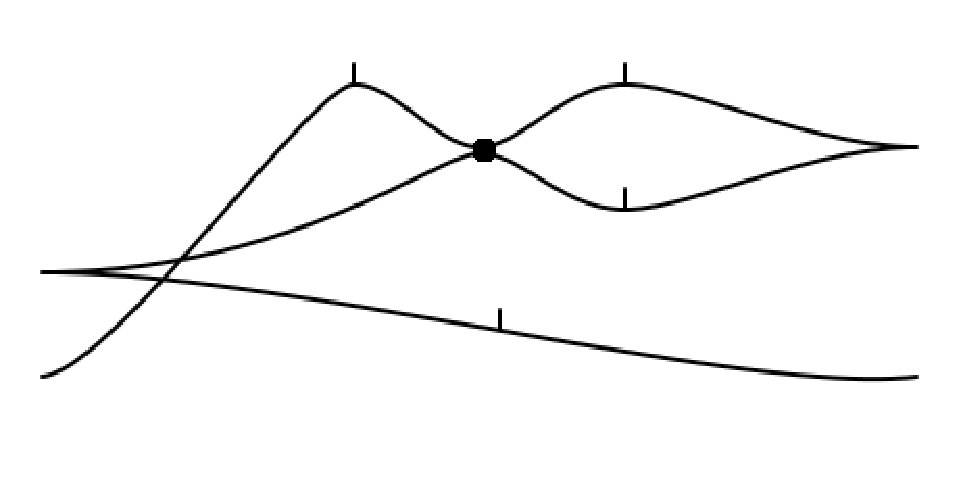
\includegraphics[width=6cm]{DoublePoint}
	\caption{A local double point in a virtual Legendrian knot.}
	\label{DoublePoint.fig}
\end{figure}

To obtain the result we will begin with $x(K_1)$ and after adding in terms on which $x$ is zero and rearranging we will change the argument of $x$ to $K_2$ withouth changing the value of $x$.  Before we begin this long string of equalities we make some observations that will be used in the manipulations:
\begin{enumerate} 
\item $x(K_1) = x(\sum_{k=0}^p(-1)^k\binom{p}{k}K_1^{k(n+1)})$, since for $k>0$, $K_1^{k(n+1)}$ has at least $n+1$ double points.  
\item $x(K_1^{m,m}) = x(K_2^{m,m})$ for $m\geq p$ as you can change $K_1^{p,p}$ to $K_2^{p,p}$ through a virtual Legendrian isotopy
\item $x(K^l) = \sum_{j=0}^{l}(-1)^j\binom{l}{j}x\left(K_1^{j,j}\right)$ as noted above.
\end{enumerate}

\begin{align*}
x(K_1) &= \sum_{k=0}^p(-1)^k\binom{p}{k} x\left( K_1^{k(n+1)}\right)& \text{by (1) above}\\
&= \sum_{k=0}^p(-1)^k\binom{p}{k}\left(\sum_{j=0}^{k(n+1)}(-1)^j\binom{k(n+1)}{j}x\left(K_1^{j,j}\right)\right)& \text{by (3) above}\\
&= \sum_{j=0}^{p(n+1)} \left( \sum_{k=\lceil\frac{i}{n+1}\rceil}^p (-1)^{k+j}\binom{p}{k}\binom{k(n+1)}{j} \right) x\left(K_1^{j,j}\right)&\\
&= \sum_{j=p}^{p(n+1)} \left( \sum_{k=\lceil\frac{i}{n+1}\rceil}^p (-1)^{k+j}\binom{p}{k}\binom{k(n+1)}{j} \right) x\left(K_1^{j,j}\right)& \text{by } \ref{comboLem}\\
&= \sum_{j=p}^{p(n+1)} \left( \sum_{k=\lceil\frac{i}{n+1}\rceil}^p (-1)^{k+j}\binom{p}{k}\binom{k(n+1)}{j} \right) x\left(K_2^{j,j}\right)& \text{by  (2) above} \\
&= \sum_{j=0}^{p(n+1)} \left( \sum_{k=\lceil\frac{i}{n+1}\rceil}^p (-1)^{k+j}\binom{p}{k}\binom{k(n+1)}{j} \right) x\left(K_2^{j,j}\right)&\\
&= \sum_{k=0}^p(-1)^k\binom{p}{k}\left(\sum_{j=0}^{k(n+1)}(-1)^j\binom{k(n+1)}{j}x\left(K_2^{j,j}\right)\right)&\\
&= \sum_{k=0}^p(-1)^k\binom{p}{k}x\left(K_2^{k(n+1)}\right)&\text{by (3) above}\\
&= x(K_2)
\end{align*} 
\qed


\begin{thm}
Let $x\in \mathcal{V}_n^\mathcal{L}$, $(F_1, K_1), (F_2, K_2) \in \mathcal{L}$ and $(F_1, K_1)$ framed isotopic to $(F_2, K_2)$ then $x(F_1, K_1) = x(F_2, K_2)$.
\end{thm}
